\documentclass[UTF8]{ctexart}
\usepackage{amsmath, enumerate, float, amssymb, lmodern}
\numberwithin{equation}{section}
\usepackage{multirow} %用于跨行
\usepackage{graphicx}%这是一个图片宏包,可处理图片的尺寸
\usepackage{float}
\usepackage{amssymb}

\usepackage{fancybox}
\usepackage{algorithm}
\usepackage{algorithmic}
\usepackage[colorlinks,
            linkcolor=black,
            anchorcolor=green,
            citecolor=blue]{hyperref}%这个宏包是用于实现跳转功能的

\usepackage{geometry}
\geometry{a4paper,scale=0.8}


\renewcommand{\algorithmicrequire}{ \textbf{Input:}} %Use Input in the format of Algorithm
\renewcommand{\algorithmicensure}{ \textbf{Output:}} %Use Output in the format of Algorithm
\renewcommand{\algorithmicrepeat}{ \textbf{Loop:}} %Use Loop in the format of Algorithm

\title{机器学习笔记}
\author{Yuxuan Yuan \& Lulu Cao}
\date{2022.2.21}
\begin{document}
\maketitle

\newpage
\tableofcontents

\newpage

\section{Lecture 1}
2022.2.21
第一节课是在C103上的,啥也没带oh
lambda 含义


\newpage
\section{Lecture 2}
2022.2.28
yyx忘了记录板书 oh

\subsection{课堂回顾}
\paragraph{机器学习=lambda} 
 : 机器 = 函数;学习 = 拟合 \newline   
Machine Learning = LAMBDA. Loss,Algorithm, Model, BigData, Application。

\textbf{BigData} $D=\{( \boldsymbol{x}_{n},y_n)\}_{n=1}^{N}$,其中$x_n \in R^N$,$y\in R$
\begin{equation*}
    \boldsymbol{y}=\left[\begin{array}{l}
                            y_{1} \\
                            y_{2} \\
                            \vdots \\
                            y_{N}
                        \end{array}\right]
        \ ,  \ \ \
    \boldsymbol{w}=\left[\begin{array}{l}
                            w_{1} \\
                            w_{2} \\
                            \vdots \\
                            w_{d}
                        \end{array}\right]
        \ ,  \ \ \
    \boldsymbol{X}=\left[\begin{array}{c}
                            \boldsymbol{x}_{1}^{\mathrm{T}} \\
                            \boldsymbol{x}_{2}^{\mathrm{T}} \\
                            \vdots \\
                            \boldsymbol{x}_{N}^{\mathrm{T}}
                        \end{array}\right]
\end{equation*}

\textbf{Model}  
\begin{equation*}
    y=\boldsymbol{w^Tx}    
\end{equation*}

\textbf{Loss} 
\begin{equation*}
    \mathcal{L}_2(\boldsymbol{w})=\frac{1}{N} \sum_{n=1}^{N}\left(y_{n}-\boldsymbol{w}^{\mathrm{T}} \boldsymbol{x}_{n}\right)^{2}    
\end{equation*}
将上述式子矩阵化,
\begin{equation*}
    \begin{aligned}
		\mathcal{L}_2(\boldsymbol{w}) &=\frac{1}{N}(\boldsymbol{X} \boldsymbol{w}-\boldsymbol{y})^{\mathrm{T}}(\boldsymbol{X} \boldsymbol{w}-\boldsymbol{y}) \\
		&=\frac{1}{N}\left((\boldsymbol{X} \boldsymbol{w})^{\mathrm{T}}-\boldsymbol{y}^{\mathrm{T}}\right)(\boldsymbol{X} \boldsymbol{w}-\boldsymbol{y}) \\
		&=\frac{1}{N}(\boldsymbol{X} \boldsymbol{w})^{\mathrm{T}} \boldsymbol{X} \boldsymbol{w}-\frac{1}{N} \boldsymbol{y}^{\mathrm{T}} \boldsymbol{X} \boldsymbol{w}-\frac{1}{N}(\boldsymbol{X} \boldsymbol{w})^{\mathrm{T}} \boldsymbol{y}+\frac{1}{N} \boldsymbol{y}^{\mathrm{T}} \boldsymbol{y} \\
		&=\frac{1}{N} \boldsymbol{w}^{\mathrm{T}} \boldsymbol{X}^{\mathrm{T}} \boldsymbol{X} \boldsymbol{w}-\frac{2}{N} \boldsymbol{w}^{\mathrm{T}} \boldsymbol{X}^{\mathrm{T}} \boldsymbol{y}+\frac{1}{N} \boldsymbol{y}^{\mathrm{T}} \boldsymbol{y}
		\end{aligned}
\end{equation*}

\textbf{Algorithm} 对损失函数求导,并令其等于0
\begin{equation*}
    \begin{aligned}
		\frac{\partial \mathcal{L}_2}{\partial w} &=\frac{2}{N} \boldsymbol{X}^{\mathrm{T}} \boldsymbol{X} \boldsymbol{w}-\frac{2}{N} \boldsymbol{X}^{\mathrm{T}} \boldsymbol{y}=0 \\
		\boldsymbol{X}^{\mathrm{T}} \boldsymbol{X} \boldsymbol{w} &=\boldsymbol{X}^{\mathrm{T}} \boldsymbol{y}
		\end{aligned}
\end{equation*}

\textbf{矩阵求导相关}
\begin{center} 
    \shadowbox{\parbox{0.5\linewidth}{
        \begin{equation*}
            \begin{array}{c|c}
                f(w) & \frac{\partial f}{\partial w} \\
                \hline w^{\mathrm{T}} \boldsymbol{x} & \boldsymbol{x} \\
                \boldsymbol{x}^{\mathrm{T}} w & \boldsymbol{x} \\
                w^{\mathrm{T}} w & 2 w \\
                w^{\mathrm{T}} \boldsymbol{C} w & 2 \boldsymbol{C} w \\
                \hline
            \end{array}
        \end{equation*}
    }}
\end{center}
从而,
\begin{equation*}
    \boldsymbol{w}=\left(\boldsymbol{X}^{\mathrm{T}} \boldsymbol{X}\right)^{-1} \boldsymbol{X}^{\mathrm{T}} \boldsymbol{y}
\end{equation*}

\subsection{投影矩阵 \& Normal Equation}

\subsection{增加新的数据(样本数 or 特征维度)}
作为作业,当$\boldsymbol{X}$增加一行(样本数增加) 或者 增加一列(特征维度增加) 时,$\boldsymbol{W}$ 如何变化,
写出更新后的$\boldsymbol{W}$和更新前的$\boldsymbol{W}$之间的增量表达式。

\textbf{相关公式}
\begin{center} 
    \shadowbox{\parbox{\linewidth}{
        \begin{itemize}
            \item \textbf{Sherman-Morrison公式} \begin{equation*}
                \left(A+u v^{T}\right)^{-1}=A^{-1}-\frac{A^{-1} u v^{T} A^{-1}}{1+v^{T} A^{-1} u}
            \end{equation*}
            \item \textbf{分块矩阵求逆}  ~ 设 $A$ 是 $m \times m$ 可逆矩阵, $B$ 是 $m \times n$ 矩阵, 
            $C$ 是 $n \times m$ 矩阵, $D$ 是 $n \times n$ 矩阵, $D-C A^{-1} B$ 是 $n \times n$ 可逆矩阵, 则有 
            \begin{equation*}
                \left[\begin{array}{ll}
                    A & B \\
                    C & D
                    \end{array}\right]^{-1}=\left[\begin{array}{cc}
                    A^{-1}+A^{-1} B\left(D-C A^{-1} B\right)^{-1} C A^{-1} & -A^{-1} B\left(D-C A^{-1} B\right)^{-1} \\
                    -\left(D-C A^{-1} B\right)^{-1} C A^{-1} & \left(D-C A^{-1} B\right)^{-1}
                    \end{array}\right]
            \end{equation*}
        \end{itemize}
        
    }}
\end{center}

\subsection{人工智能的流派}
\begin{itemize}
    \item 类比主义:核方法、SVM
    \item 连接主义:神经网络
    \item 贝叶斯主义
    \item 符号主义:决策树、专家系统
    \item 演化主义(优化算法):遗传算法
    \item 行为主义:强化学习
\end{itemize}

\subsection{人脸识别}
设$D$为人脸的数据, $D=\{( \boldsymbol{x}_{n},y_n)\}_{n=1}^{N}$,
其中$x_n \in R^N$,$y\in [1,100]$, $y_i=w^Tx_i+\epsilon,\epsilon\sim W(0,\sigma^2) $,$\sigma^2=1$,
则$y_i \sim W(w^Tx_i,1)$

方差一样,所以一样胖;均值不一样,所以location不同

找到一个$w$,使得$y_i$出现的概率最大, 即$P(y_i|w^Tx,1)=\frac{1}{\sqrt{2\pi}}exp{-\frac{1}{2}(\frac{y_i-w^Tx}{1})^2}$
\begin{equation*}
    L=p\left(\boldsymbol{y} \mid \boldsymbol{X}, w, \sigma^{2}\right)=\prod_{n=1}^{N} p\left(y_{n} \mid \boldsymbol{x}_{n}, w, \sigma^{2}\right)=\prod_{n=1}^{N} \mathcal{N}\left(w^{\mathrm{T}} \boldsymbol{x}_{n}, \sigma^{2}\right)
\end{equation*}
取对数, 有 
\begin{equation*}
    \begin{aligned}
        \log L &=\sum_{n=1}^{N} \log \left(\frac{1}{\sqrt{2 \pi \sigma^{2}}} \exp \left\{-\frac{1}{2 \sigma^{2}}\left(y_{n}-f\left(\boldsymbol{x}_{n} ; \boldsymbol{w}\right)\right)^{2}\right\}\right) \\
        &=\sum_{n=1}^{N}\left(-\frac{1}{2} \log (2 \pi)-\log \sigma-\frac{1}{2 \sigma^{2}}\left(y_{n}-f\left(\boldsymbol{x}_{n} ; w\right)\right)^{2}\right) \\
        &=-\frac{N}{2} \log 2 \pi-N \log \sigma-\frac{1}{2 \sigma^{2}} \sum_{n=1}^{N}\left(y_{n}-f\left(\boldsymbol{x}_{n} ; w\right)\right)^{2}
    \end{aligned}
\end{equation*}

$w^{\mathrm{T}} \boldsymbol{x}_{n}$ 替换模型中的决定性部分, 对数似然表达式就呈现如下的形式: $\log L=-\frac{N}{2} \log 2 \pi-N \log \sigma-\frac{1}{2 \sigma^{2}} \sum_{n=1}^{N}\left(y_{n}-w^{\mathrm{T}} \boldsymbol{x}_{n}\right)^{2}$
得到的最小二乘解, 通过求导数、使其等于零以及求解拐点的方法, 类似于 $1.1 .4$ 节所述的方式。对于 $w$ (注意, $w^{\mathrm{T}} \boldsymbol{x}_{n}=\boldsymbol{x}_{n}^{\mathrm{T}} \boldsymbol{w}$ ),

最小二乘法和极大似然估计是等价的
\newpage

\section{Lecture 3}
2022.3.7

\textbf{Outline}
\begin{enumerate}
    \item Least Square: MLE 
    \begin{enumerate}
        \item[1.1] SGD
        \item[1.2] Probalistic Graph Representation
        \item[1.3] $ \mathbb{E}[\hat w] / cov[\hat w] $
        \item[1.4] bias / variance
    \end{enumerate}
    
    \item Revisted LS: Curve Fitting
    \begin{enumerate}
        \item[2.1] Model Selection
        \item[2.2] Overfitting
    \end{enumerate}
    \item How to solve overfitting
    \begin{enumerate}
        \item[3.1] Regularization (MAP)
        \item[3.2] Bayesian Learning
    \end{enumerate}
\end{enumerate}

\newpage
\section{Lecture 4}
2022.3.14

使用MLE/MAP/Bayes Learning三种方法来求解参数,通过4个例子来加深。Example 4没讲完。
其中Example 3的三种解法需要自己课后补充。

tips: to be added
三个图 对应生成式模型、判别式模型、分布计算;
一些前置 discrete continuous 的概率表 变量分布;
有积分的地方 和 是求谁的期望的地方,


\textbf{Outline}
\begin{itemize}
    \item MLE / MAP / Bayesian
    \item Example 1. Bernoulli
    \item Example 2. Gaussian
    \item Example 3. Linear Regression
    \item Example 4. Logistic Regression
\end{itemize}
问题:
\begin{itemize}
    \item 共轭分布是什么意思
    \item $\beta$分布
\end{itemize}

\subsection{Example 1. Bernoulli}
Given dataset $D=\{<x_i>\}_{i=1}^n, x_i \in \{0,1\}$
$x_i$服从Bernoulli分布,$P(x_i=1)=\theta$;
再假设$n_1$表示$D$中$x_i=1$的个数;

\textbf{Method}

1. MLE 
\begin{align*}
    P(D|\theta) &= \prod_{i=1}^n P(x_i; \theta) \\
    &= \prod_{i=1}^n \theta^{x_i} (1-\theta)^{1-x_i} \\
    &= \theta^{\sum_i x_i} (1-\theta)^{n-\sum_i x_i} \\
    &= \theta^{n_1} (1-\theta)^{n-n_1} \\
\end{align*}
取对数以便计算,从而
\begin{align*}
    \underset {\theta} {\arg \max} \ln P(D|\theta) &= \underset {\theta} {\arg \max} n_1 \ln \theta + (n-n_1) \ln (1-\theta) \\
\end{align*}
对$\theta$求导
\begin{equation*}
    \frac{n_1}{\theta} - \frac{n-n_1}{1-\theta} = 0
\end{equation*}
得到 $\theta = \frac{n_1}{n}$


2. MAP

Beta分布 $Beta(\theta \mid a, b)$
$P(\theta | D) \propto P()$ 

\begin{center} 
\shadowbox{\parbox{\linewidth}{
    贝塔分布(Beta Distribution) 是一个作为伯努利分布和二项式分布的共轭先验分布的密度函数。在概率论中,贝塔分布,也称Β分布,是指一组定义在(0,1) 区间的连续概率分布。    
}}
\end{center}

3. Bayesian


\subsection{Example 2. Gaussian}

\textbf{Method}

1. MLE 

2. MAP

3. Bayesian

\subsection{Example 3. Linear Regression}
Given dataset $D=\{<x_i, y_i>\}_{i=1}^n, y_i \in \mathbb{R}$,
假设 $X ~ \mathcal{N}(\theta, \sigma^2)$,则有
$P(x;\theta) = \frac{1}{\sigma \sqrt{2\pi}}\exp\{-\frac{(x-\theta)^2}{2\sigma^2}\}$

\textbf{Method}

1. MLE 

2. MAP

3. Bayesian

\subsection{Example 4. Logistic Regression}

\textbf{Method}

1. MLE 

2. MAP
3. Bayesian

\textbf{计算步骤(流程)总结}

\begin{enumerate}
    \item $P(D|\theta)$
    \item $P(\theta)$
    \item $P(\theta|D) \propto P(D | \theta)P(\theta)$
    \item $\theta_{bayes} = \mathbb{E}[\theta | D]$
    \item inference: $P(y_{new}|D,x_{new})=\int p(y_{new}|x_{new}, \theta)p(\theta | D)$
\end{enumerate}
其中$D = (X,Y)$


\newpage

\section{Lecture 5}
2022.3.21


\textbf{Outline}
\begin{enumerate}
    \item Review: MLE / MAP / Bayesian Estimation
    \item Logistic Regression
    \item Perceptron
    \item Generative Classification Model
        \subitem x is continuous (GDA)
        \subitem x is discrete (NB)
\end{enumerate}

\dotfill

\textbf{Data}: $D={<x_i, y_i>}_{i=1}^n, x_i \in \mathbb{R}^d, y_i\in{0,1}, D=(X,Y)$ 

\textbf{Model}: $P(x,y; \Theta)$(生成式) ; $P(y|x; \Theta)$(判别式) ; $P(x_i; \Theta)$无监督

\textbf{Inference}: Given $x, D$; Output $y$, $P(y|x, D)=?$

\textbf{Learning}: Given $D$; Output $\Theta$, $P(D|\Theta)$, $\Theta_{Bayes}=\mathbb{E}[\Theta|D]$

\dotfill

\subsection{Review: MLE / MAP / Bayesian}
三种方法,即Learning的三种方法
\subsubsection*{\textbf{Learning}} 

\textbf{1. MLE }


\begin{equation*}
    \begin{aligned}
        \hat \Theta_{MLE} &= \underset{\Theta}{\arg \max} P(D | \Theta)     \\
        &= \underset{\Theta}{\arg \max} \sum_{i=1}^n \ln P( \textit{blank} ; \Theta) \\
    \end{aligned}
\end{equation*}
其中,\textit{blank}可以填入1)$x_i, y_i$; 2)$y_i|x_i$; 3)$x_i$; 即三种模型都可用MLE求解

\textbf{2. MAP}

\begin{equation*}
    \begin{aligned}
        \hat \Theta_{MAP} &= \underset{\Theta}{\arg \max} P(\Theta | D)  \propto P(D|\Theta)P(\Theta)   \\
        &= \underset{\Theta}{\arg \max} \ln P( \textit{blank} ; \Theta) + \ln P(\Theta)\\
    \end{aligned}
\end{equation*}
其中,$P(\Theta)$是先验,$P(D|\Theta)$是似然,等式的最后$\ln P( \textit{blank} $为数据项(Data Term), 
$\ln P(\Theta)$为正则项(Regularization Term, 或平滑项(Smooth Term))。

* 当$P(\Theta)$是均匀分布时, $MLE=MAP$ 。


\textbf{3. Bayesian Estimation}

(前提是$P(\Theta | D)$即后验分布已知)

\begin{equation*}
    \hat \Theta_{Bayes} = \mathbb{E}[\Theta | D ] = E_{\theta \sim P(\cdot | D)}[\Theta] = \int \Theta p(\Theta | D) d\Theta
\end{equation*}


\subsubsection*{\textbf{Inference}}

利用上述三种方法做参数估计后的推理方法


\textbf{1. MLE}

Given $\hat \Theta_{MLE}, x, D$, ouput $P(y | x; \hat \Theta_{MLE} )$.

举例,在Logistic Regression中,$P(y=1|x;\hat \Theta_{MLE} )=\sigma({\hat \Theta_{MLE} }^T x)$

\textbf{2. MAP}

Given $\hat \Theta_{MAP}, x, D$, output $P(y | x; \hat \Theta_{MAP} )$.

举例,在Logistic Regression中,$P(y=1|x;\hat \Theta_{MAP} )=\sigma({\hat \Theta_{MAP} }^T x)$

\textbf{3.Bayes Estimation}

Given $ x, D, P(\Theta|D)$, ouput $P(y | x; \hat \Theta_{MAP} )$.
\begin{equation*}
    \begin{aligned}
        P(y|x;D) &= \int p(y, \Theta | x;D) d\Theta    \\
        &= \int p(\Theta | x;D)p(y|\Theta,x;D)d\Theta
    \end{aligned}    
\end{equation*}
等式最后的$p(\Theta | x;D)$为后验分布,$p(y|\Theta,x;D)$为模型。
能这么做的前提是假设$x_{new}$与$\Theta$无关。

如果求$y=1$, 有
\begin{equation*}
    \begin{aligned}
        p(y|\Theta,x;D)&=\int p(\Theta|D)\sigma(\Theta^T x)dx ~ (= \mathbb{E}_{{\Theta} \sim P(\cdot |D)}[\sigma(\Theta^Tx)] \\
        &\approx \frac{1}{\mathcal{L}} \sum_{i=1}^{\mathcal{L}} \sigma((\Theta^{(i)})^Tx)
    \end{aligned}
\end{equation*}
其中有假设$x_{new}$与$\Theta$相互独立;$\Theta^{(i)} \sim P(\Theta |D))), i=1,...,\mathcal{L}$, 上面公式使用了抽样技术(Sampling)来求期望。

\subsection{Logistic Regression(逻辑斯蒂回归)}
补点图 概率图模型 (可观测量用灰色阴影)

\subsubsection*{\textbf{Learning}}

\textbf{1.MLE}
\begin{equation*}
    P(y_i|x_i;\Theta) = \sigma(\Theta^T x_i)^{y_i} (1-\sigma(\Theta^Tx_i))^{1-y_i}
\end{equation*}

\begin{equation*}
    \begin{aligned}
        lnP(D|\Theta) &= \sum_{i=1}^n \{y_i\ln\sigma_i +(1-y_i)\ln(1-\sigma_i)\}    \\
        &= \mathcal{L}_D(\Theta)
    \end{aligned}
\end{equation*}
其中$\sigma_i=\sigma(a_i)=\sigma(\Theta^Tx_i)=\frac{1}{1+e^{\Theta^Tx_i}}$, 从而
\begin{equation*}
    \Theta^* = \underset{\Theta}{\arg \max} {\mathcal{L}_D(\Theta)}
\end{equation*}
到这里,求解$\Theta^*$方法有 求偏导数并等于0来计算解析解,但无法做到,原因如下,利用链式法则算一下偏导数
\begin{equation*}
    \begin{aligned}
        \nabla_\Theta \mathcal{L}_D(\Theta) &=\frac{\partial \mathcal{L}_D ( \Theta) }{\partial \Theta} \\
        &= \frac{\partial\mathcal{L}_D ( \Theta)}{\partial \sigma_i}\frac{\partial \sigma_i}{\partial a_i}\frac{\partial a_i}{\partial \Theta}\\
        &= \sum_{i=1}^n(\frac{y_i}{\sigma_i}-\frac{1-y_i}{1-\sigma_i})\sigma_i(1-\sigma_i)x_i \\
        &= \sum_{i=1}^n(y_i-\sigma_i)x_i
    \end{aligned}
\end{equation*}
试试,几乎无法求得解析解。

第二种方法,尝试二阶导数$\nabla_\Theta(\nabla_\Theta \mathcal{L}_D(\Theta) )$, 令$\nabla_\Theta \mathcal{L}_D(\Theta) =g$,

\begin{algorithm}[htb]
    \caption{A1: Gradient Ascent for Logistic Regression}
    \label{alg:A1}
    \begin{algorithmic}[1]
    \REQUIRE
    X, Y; \\
    \ENSURE 
    $\Theta$; \\
    \STATE init: $\Theta \sim \mathcal{N}(0, \alpha^{-1}\mathrm{I}), \epsilon$
    \REPEAT 
    \STATE $g=\mathbf{X}^T(\mathbf{Y}-\sigma)$
    \STATE $\Theta^{t+1} := \Theta^t + \eta g$
    \UNTIL $\mid\mid \Theta^{t+1} -\Theta^t \mid\mid \leq \epsilon$
    \RETURN $\Theta$;
    \end{algorithmic}
\end{algorithm}

\textbf{Hessian Matrix of the Loss Function $\mathcal{L}_D(\Theta)$}


\textbf{Newton}
$\Theta^{t+1} := \Theta^t + \text{H}^{-1} g$
......todo

\textbf{2.MAP}

\begin{gather*}
    P(\Theta) \sim \mathcal{N}(0, \alpha^{-1}\text{I}) \\
    P(D|\Theta) = \prod_{i=1}^n\sigma_i^{y_i}(1-\sigma_i)^{1-y_i} \\
    P(\Theta | D) \propto \mathcal{N}(0, \alpha^{-1}\text{I}) \prod_{i=1}^n\sigma_i^{y_i}(1-\sigma_i)^{1-y_i} \\
\end{gather*}
根据MAP,有
\begin{equation*}
    \begin{aligned}
        \Theta^* &= \underset {\Theta} {\arg \max} \ln{P(\Theta|D)} \\
        &= \underset{\Theta}{\arg \max} \ln P(D|\Theta) + \ln P(\Theta) \\
        &= \underset{\Theta}{\arg \max} {\sum_{i=1}^n y_i \ln(\sigma_i) + (1-y_i)\ln{(1-\sigma_i)} -\frac{1}{2}(\Theta^{-1}\Sigma^{-1}\Theta)} 
    \end{aligned}        
\end{equation*}
则
\begin{equation*}
    \begin{aligned}
        \nabla_\Theta \mathcal{L}_D(\Theta) &=\frac{\partial \mathcal{L}_D ( \Theta) }{\partial \Theta} \\
        &= \sum_{i=1}^n(y_i-\sigma_i)x_i - \Theta \Sigma^{-1} 
    \end{aligned}
\end{equation*}
这里 定$\alpha^{-1}\mathrm{I} = \Sigma$,不影响结果。

类似算法\text{A1},写个\text{A2}

\
\begin{algorithm}[htb]
    \caption{A2: (MAP) Gradient Ascent for Logistic Regression}
    \label{alg:A2}
    \begin{algorithmic}[1]
    \REQUIRE
    X, Y; \\
    \ENSURE 
    $\Theta$; \\
    \STATE init: $\Theta \sim \mathcal{N}(0, \alpha^{-1}\mathrm{I}), \epsilon$
    \REPEAT 
    \STATE $g=\mathbf{X}^T(\mathbf{Y}-\sigma) - \Theta^t\Sigma^{-1}$
    \STATE $\Theta^{t+1} := \Theta^t + \eta g$
    \UNTIL $\mid\mid \Theta^{t+1} -\Theta^t \mid\mid \leq \epsilon$
    \RETURN $\Theta$;
    \end{algorithmic}
\end{algorithm}

\textbf{3.Bayesian Estimation}

贝叶斯估计:
$\mathbb{E}[\Theta | D]$

$P(y=1|x, D) = $
类似算法\text{A1},写个\text{A3}用于贝叶斯推理

Inference
后验预测分布为
\begin{equation*}
    p(y=1|x_{new}, D) = \int p(y=1 | x_{new}, \Theta)p(\Theta|x,D)d\Theta
\end{equation*}
但是积分难以处理,采用近似处理,同时还有假设$x_{new}$与$\Theta$无关,有
\begin{equation*}
    \begin{aligned}
        p(y=1|x_{new}, D) &= \int p(y=1 | x_{new}, \Theta, D)p(\Theta|D)d\Theta \\
        &= \int \sigma(\Theta^Tx_{new})p(\Theta |D)d\Theta \\
        &\approx \frac{1}{\mathcal{L}}\sum_{i=1}^{\mathcal{L}} \sigma((\Theta^{(i)})^Tx_{new} )
    \end{aligned}
\end{equation*}
其中,${\Theta}^{(i)} \propto p(\Theta | D) (i=1,..., \mathcal{L})$

\begin{algorithm}[htb]
    \caption{A3: Inference after Bayesian Estimation}
    \label{alg:A3}
    \begin{algorithmic}[1]
    \REQUIRE
    $x_{new}$, D; \\
    \ENSURE 
    y; \\
    \STATE init: ${\Theta}^{(i)} \propto p(\Theta | D) (i=1,..., \mathcal{L})$
    \STATE $P(y=1|x_{new},D)=\frac{1}{\mathcal{L}} \sum_{i=1}^{\mathcal{L}} \sigma((\Theta^{(i)})^T x_{new})$
    \STATE $P(y=0|x_{new},D)=\frac{1}{\mathcal{L}}\sum_{i=1}^{\mathcal{L}} (1-\sigma((\Theta^{(i)})^Tx_{new}) )$
    \RETURN 1 if $P(y=1|x_{new},D) > P(y=0|x_{new},D)$ else 0;
    \end{algorithmic}
\end{algorithm}


\subsection{Perceptron(感知机)}

写个历史表
\begin{itemize}
    \item 1943 M-P ----神经元模型
    \item 1957 Rosenblatt ----Perceptron;
    \item 1982 BP算法(Computational Graph计算图)
    \item 2006 Hinton ----预训练pretain、DNN
    \item 2012 AlexNet....图像不太懂...
\end{itemize}

\textbf{Model}

计算方法:$y=sgn(\mathbf{W}^Tx+b)$

其中;
\begin{equation*}
    \left\{ \begin{aligned}
        y=+1, &\mathbf{W}^Tx+b > 0 , \\ 
        y=-1, &\mathbf{W}^Tx+b<0 
    \end{aligned}
    \right.
\end{equation*}

\textbf{Loss计算}

\begin{equation*}
    \mathcal{L}_D(W) = \sum_{x_i, y_i \in M} \frac{|y_i (W^Tx_i+b)|}{||W||}
\end{equation*}
其中 $M = \{(x_i, y_i) | y_i(W^Tx+b)<0\}$,可令$||W||=1$,上式可写成,
\begin{equation*}
    \mathcal{L}_D(W) = \sum_{i=1}^n\max\{0, -y_i(W^Tx_i+b)\} 
\end{equation*}
* 当$\max$中的第二项变为$1-y_i(W^Tx_i+b)$时,损失函数变成SVM的损失函数。

这里求一下偏导数,对于单个样本$(x_i, y_i)$
\begin{equation*}
    \frac{\partial (-y_i(W^Tx_i + b))}{\partial W} = -y_i x_i
\end{equation*}
也可以写成一个算法形式

\begin{algorithm}[htb]
    \caption{A4: Perceptron GD}
    \label{alg:A4}
    \begin{algorithmic}[1]
    \REQUIRE
    $X, Y$; \\
    \ENSURE 
    $\Theta=\{W, b\}$; \\
    \STATE init: $W, b$
    \REPEAT 
    \IF{$y_i(W^T x_i + b) < 0 $}
        \STATE {$W^{t+1} \leftarrow W^t - \eta \nabla_W {\mathcal{L}_D(W)}$}
        \STATE 等价于 $W^{t+1} \leftarrow W^t + \eta y_i x_i$
    \ENDIF
    \UNTIL 训练集中没有误分类点
    \RETURN $\Theta$;
    \end{algorithmic}
\end{algorithm}


\subsection{Generative Classification Model}
\subsubsection*{$y$ 是离散的}

\textbf{x是连续的} 

Given $\{(x_i, y_i)\}_{i=1}^n = D = (X, Y), x\in \mathbb{R}^d$。
假设$y_i={0, 1}$,即$y_i$服从Bernoulli分布,$x_i$服从高斯分布$x_i|y_i \sim \mathcal{N}(\mu_k, \Sigma_k)$,model描述如下
\begin{equation*}
    \begin{aligned}
        P(x_i, y_i; \Theta) &= P(y_i; \Theta) P(x_i|y_i;\Theta) \\
        &= \text{Bernoulli}(y_i|p)  \prod_{y=0}^1\mathcal{N}(x_i | \mu_k, \Sigma_k)^{\mathbf{1}\{k=y\}}
    \end{aligned}
\end{equation*}
关于$P(x_i|y_i;\Theta)$部分细述如下,
\begin{gather*}
    P(x|y=1; \Theta) = \mathcal{N}(x|\mu_1, \Sigma_1) \\
    P(x|y=0; \Theta) = \mathcal{N}(x|\mu_0, \Sigma_0) \\
\end{gather*}
从而有
\begin{equation*}
    P(x|y;\Theta) = \mathcal{N}(x|\mu_1, \Sigma_1)^{\mathbf{1}\{y=1\}} \mathcal{N}(x|\mu_0, \Sigma_0)^{\mathbf{1}\{y=0\}}
\end{equation*}
记$\Theta=(p, \mu_0,\Sigma_0, \mu_1, \Sigma_1)$,则有
\begin{equation*}
    \begin{aligned}
        P(D;\Theta) &= \prod_{i=1}^n P(x_i, y_i; \Theta) \\
        &= \prod_{i=1}^n (p^{y_i}(1-p)^{1-y_i}) \mathcal{N}(x|\mu_1, \Sigma_1)^{\mathbf{1}\{y=1\}} \mathcal{N}(x|\mu_0, \Sigma_0)^{\mathbf{1}\{y=0\}}
    \end{aligned}
\end{equation*}
取对数,有
\begin{equation*}
    \begin{aligned}
        \ln P(D;\Theta) &= \sum_{i=1}^n y_i\ln p+ (1-y_i) \ln (1-p) + \sum_{i=1}^n {\mathbf{1}\{y=1\}} \ln{\mathcal{N}(x_i|\mu_1, \Sigma_1)}+\sum_{i=1}^n{\mathbf{1}\{y=0\}} \ln{\mathcal{N}(x_i|\mu_0, \Sigma_0)}
    \end{aligned}
\end{equation*}

Learning time !!!!!
\textbf{MLE}
 
根据$\hat \Theta_{MLE}=\underset{\Theta}{\arg \max}\ln{P(D;\Theta)}$, 假设$\Sigma_0, \Sigma_1$已知,
设$M_1=\{(x_i, y_i)| y_i=1\}, M_0=\{(x_i, y_i)| y_i=0\}$,
求$p, \mu_0, \mu_1$。
\begin{gather*}
    \mathcal{L}_D(\Theta) = \ln{P(D;\Theta)} \\
    \ln{\mathcal{N}(x|\mu,\Sigma)} = -\frac{d}{2}\ln{(2\pi)}-\frac{1}{2}\ln{|\Sigma|}-\frac{1}{2}(x-\mu)^T\Sigma^{-1}(x-\mu) \\
    \frac{\partial \mathcal{L}_D(\Theta)}{\partial p} = \sum_{i=1}w^n(\frac{y_i}{p}-\frac{1-y_i}{1-p}) =0 \\
    \frac{\partial \mathcal{L}_D(\Theta)}{\partial \mu_0} =  \sum_{(x_i,y_i)\in M_0} {\Sigma^{-1}(x_i-\mu_0)} =0 \\
    \frac{\partial \mathcal{L}_D(\Theta)}{\partial \mu_1} =  \sum_{(x_i,y_i)\in M_1} {\Sigma^{-1}(x_i-\mu_1)} =0 \\
\end{gather*}

解得
\begin{gather*}
    p = \frac{\sum_{i=1}^n y_i}{n} \\
    \mu_0 = \frac{\sum_{(x_i, y_i)\in M_0}x_i}{|M_0|} \\
    \mu_1 = \frac{\sum_{(x_i, y_i)\in M_1}x_i}{|M_1|} 
\end{gather*}

Infering time !!!

Given $x, y=?$, $p, \mu_0, \mu_1, \Sigma_0, \Sigma_1$ are known.

\begin{gather*}
    \begin{aligned}
        P(y=1|x) & \propto P(y=1)P(x|y=1) \\    
        &=p \mathcal{N}(x|\mu_1, \Sigma_1) \\
    \end{aligned}
    \\
    \begin{aligned}
        P(y=0|x) & \propto P(y=0)P(x|y=0) \\    
        &=(1-p) \mathcal{N}(x|\mu_0, \Sigma_0) 
    \end{aligned}
\end{gather*}
若$ P(y=1|x) >  P(y=0|x)$ ,则$y=1$。

\subsection{\textbf{作业} }
\begin{gather*}
    \begin{aligned}
        g(x) &=\ln{\frac{P(y=1|x)}{P(y=0|x)}} \\     
        &=\ln{\frac{p \mathcal{N}(x|\mu_1, \Sigma_1)}{(1-p) \mathcal{N}(x|\mu_0, \Sigma_0) }}
    \end{aligned}
\end{gather*}

设$ \Sigma_1=\Sigma_0 $, 则$g(x)$是线性平面,可写作$g(x) = w^Tx+b$,即 Gaussian Discriminative Analysis(GDA),
求$w, b$
\begin{equation*}
    \begin{aligned}
        g(x) &= \ln{\frac{p}{1-p}} + (\frac{1}{2}((x-\mu_0)^T\Sigma^{-1}(x-\mu_0)-(x-\mu_1)^T\Sigma^{-1}(x-\mu_1))) \\
        & = \ln{\frac{p}{1-p}} + \frac{1}{2}((x^T-{\mu_0}^T)\Sigma^{-1}(x-\mu_0) - (x^T-{\mu_1}^T)\Sigma^{-1}(x-\mu_1))))\\
        &= \ln{\frac{p}{1-p}} + \frac{1}{2}(x^T \Sigma^{-1}x - x^T\Sigma^{-1}\mu_0 - {\mu_0}^T\Sigma^{-1}x + {\mu_0}^T\Sigma^{-1}\mu_0 + x^T \Sigma^{-1}x + x^T\Sigma^{-1}\mu_1 + {\mu_1}^T\Sigma^{-1}x - {\mu_1}^T\Sigma^{-1}\mu_1) \\
        &= \ln{\frac{p}{1-p}} + \frac{1}{2}(2({\mu_1}^T \Sigma^{-1}x - {\mu_0}^T \Sigma^{-1}x) + {\mu_0}^T\Sigma^{-1}\mu_0 - {\mu_1}^T\Sigma^{-1}\mu_1) \\
        &= ({{\mu_1}-{\mu_0}})^T\Sigma^{-1}x + \frac{1}{2}{\mu_0}^T\Sigma^{-1}\mu_0 - \frac{1}{2}{\mu_1}^T\Sigma^{-1}\mu_1 + \ln p - \ln{(1-p)} 
    \end{aligned}
\end{equation*}
即 (结合:$w$记得算一下转置,$\Sigma$是对称矩阵等内容)
\begin{gather*}
    w = \Sigma^{-1}({{\mu_1}-{\mu_0}})\\
    b = \frac{1}{2}{\mu_0}^T\Sigma^{-1}\mu_0 - \frac{1}{2}{\mu_1}^T\Sigma^{-1}\mu_1 + \ln p - \ln{(1-p)}  
\end{gather*}

\paragraph*{x是离散的}

\newpage
\section{Lecture 6}
2022.3.28


\textbf{Outline}
\begin{enumerate}
    \item Generative Classification Model : $p(x,y)$, y is discrete
        \subitem x is continuous (高斯判别分析 GDA)
        \subitem x is discrete (朴素贝叶斯 NB)
    \item 贝叶斯学习
\end{enumerate}

\subsection{朴素贝叶斯 NB}
\dotfill

Problem: $D=\{( \boldsymbol{x}_{i},y_i)\}_{i=1}^{n}$,其中$x_i \in R^d$,$y_i\in \{0,1\}$,  $<X,Y> \sim P$

\dotfill

\subsubsection{原理与模型}

假设:各个维度独立;每个维度的取值为0或1
$$
P(X_1,...,X_d|Y)=\prod^d_{j=1}P(X_j|Y)
$$

\dotfill

 条件独立:$P(X|Y,Z)=P(X|Z)=X\perp Y|Z$
 
 $P(X|Y)=P(X_1,X_2|Y)=P(X_1|X_2,Y)P(X_2|Y)=P(X_1|Y)P(X_2|Y)$
 
 \dotfill

模型:
$$
\begin{aligned}
y^*(分类结果)&=\underset{y_k}{\arg \max } \frac{P(y_k)P(X|y_k)}{P(X)}\\
&=\underset{y_k}{\arg \max }~{P(Y=y_k)\prod_{j=1}^d P(X_j=x_j|Y=y_k)}\\
\end{aligned}
$$



\subsubsection{算法}
\begin{enumerate}
    \item MLE
    
    其实就是计算频率
    \item 零频率问题

解决方案:拉普拉斯平滑
$$
P(w \mid c)=\frac{\operatorname{num}(w, c)+\varepsilon}{\operatorname{num}(c)+k \varepsilon}
$$
PS:属性缺失不用管

\end{enumerate}


\subsubsection{小结:产生式p(y|x) vs. 判别式p(x,y)}
\begin{enumerate}
    \item 产生式模型有其对应的判别式模型,这样的组合叫做“产生式-判别式”对;(e.g. 根据p(x,y)得到GDA的分界面);
    \item 判别式模型不一定有其对应的产生式模型;
    \item 训练样本多的情况下,采用判别式;
    \item 训练样本少的情况下,选择产生式。
\end{enumerate}

\subsection{贝叶斯学习}
\begin{enumerate}
    \item MLE/MAP/贝叶斯估计
    \item 贝叶斯估计:将先验信息集成到模型推理中 $p(x,X,\theta)$
\end{enumerate}

\subsection*{\textbf{作业} }
朴素贝叶斯的贝叶斯估计

输入: 训练集 $T=\left\{\left(x_{1}, y_{1}\right),\left(x_{2}, y_{2}\right), \ldots\left(x_{N}, y_{N}\right)\right\}$, 其中 $x_{i}=\left(x_{i}^{(1)}, x_{i}^{(2)}, \ldots, x_{i}^{(n)}\right)^{T}$ ,第 $\mathrm{i}$ 个样本的第 $\mathrm{j}$ 个特征$x_{i}^{(j)}$可能的取值集合为 $\left\{a_{j 1}, a_{j 2}, \ldots, a_{j S_{j}}\right\}$ ,即某一特征的取值为有限集合。
$y_{i} \in\left\{c_{1}, c_{2}, \ldots, c_{K}\right\}$ , 即分类结果为有限集合 (共 $\mathrm{K}$ 个)。

先验概率的贝叶斯估计为:
$$
P\left(Y=c_{k}\right)=\frac{\sum_{i=1}^{N} I\left(y_{i}=c_{k}\right)+\lambda}{N+K\lambda}, k=1,2, \ldots, K
$$

条件概率的贝叶斯估计为:
$$
P\left(X^{(j)}=a_{j l} \mid Y=c_{k}\right)=\frac{\sum_{i=1}^{N} I\left(x_{i}^{(j)}=a_{j l}, y_{i}=c_{k}\right)+\lambda}{\sum_{i=1}^{N} I\left(y_{i}=c_{k}\right)+S_j\lambda}
$$

朴素贝叶斯的贝叶斯估计为:
$$
y=\underset{c_k}{\arg \max}P(Y=c_{k})\prod_{j=1}^nP(X^{(j)}=x_{j }\mid  Y=c_{k})
$$

\newpage
\section{Lecture 7}
2022.4.4

\textbf{Outline}
\begin{enumerate}
    \item 狄利克雷分布
    \item MLE/MAP/Bayesian Learning:多分类
    \item Bernoulli Mixture Model
    \item EM算法
        \subitem EM-principle
        \subitem EM-convergence
        \subitem EM for GMM
        \subitem EM for Topic Model
\end{enumerate}

\subsection{狄利克雷分布}

\subsubsection{二项分布}
二项分布用以描述 $n$ 次独立的伯努利实验中有 $m$ 次成功的概率:
$$
\begin{aligned}
P(X=m)=\binom{n}{m} p^{m}(1-p)^{n-m}
\end{aligned}
$$
当试验的次数n为1时,二项分布变成伯努利分布。

\subsubsection{多项分布}
多项分布是一种多元离散随机变量的概率分布,是二项分布的扩展。
假设重复进行n次独立随机试验,每次试验可能出现的结果有k种,第$i$
种结果出现的概率为$p_i$,第$i$种结果出现的次数为$n_i$。如果用随机变量
$X=(X_1,X_2,...,X_k)$表示试验所有可能结果的次数,其中$X_i$表示第$i$种结果出现的次数,
那么随机变量X服从多项分布。

$$
\begin{aligned}
    P\left(X_{1}=n_{1}, \cdots, X_{k}=n_{k}\right)&= \frac{n !}{n_{1} ! \cdots n_{k} !} p_{1}^{n_{1}} \cdots p_{k}^{n_{k}} ~~~~ , \sum_{i=1}^{k} n_{i}=n \\ 
&=n ! \prod_{i=1}^{k} \frac{p_{i}^{n_{i}}}{n_{i} !} ~~~~ , \sum_{i=1}^{k} n_{i}=n \\ 
\end{aligned}
$$
当试验的次数n为1时,多项分布变成类别分布。类别分布表示试验可能出现的k种结果的概率。

\subsubsection{贝塔分布}
贝塔分布是关于连续变量 $x \in[0,1]$ 的概率分布,它由两个参数 $a>0$ 和 $b>0$ 确定:
$$
\begin{aligned}
\operatorname{Beta}(x \mid a, b)=\frac{\Gamma(a+b)}{\Gamma(a) \Gamma(b)} x^{a-1}(1-x)^{b-1}=\frac{1}{B(a, b)} x^{a-1}(1-x)^{b-1}
\end{aligned}
$$

其中, $\Gamma(s)$ 为Gamma函数:
$$
\begin{aligned}
\Gamma(s)=\int_{0}^{+\infty} t^{s-1} e^{-t} d t
\end{aligned}
$$

$B(a, b)$ 为Beta函数,用来做归一化:
$$
\begin{aligned}
B(a, b)=\frac{\Gamma(a) \Gamma(b)}{\Gamma(a+b)}
\end{aligned}
$$


\subsubsection{狄利克雷分布}
狄利克雷分布是一种多元连续随机变量的概率分布,是贝塔分布的扩展。在贝叶斯学习中,
狄利克雷分布常作为多项分布的先验分布使用。
狄利克雷分布是关于一组 $d$ 个连续变量 $x_{i} \in[0,1]$ 的概率分布, $\sum_{i} x_{i}=1_{0}$ 。令 $\mu=$ $\left(\mu_{1}, \mu_{2}, \cdots, \mu_{d}\right)$ ,参数 $\alpha=\left(\alpha_{1}, \alpha_{2}, \cdots, \alpha_{d}\right)$ ,其中 $\alpha_{i}>0$ 且 $\hat{\alpha}=\sum_{i} \alpha_{i \text { 。 }}$
$$
\begin{aligned}
\operatorname{Dir}(x \mid \alpha)=\frac{\Gamma(\sum^{d}_{i=1}\alpha_i)}{\prod_{i=1}^{d}\Gamma(\alpha_i)}  \prod_{i=1}^{d}x_{i}^{\alpha_{i}-1}
\end{aligned}
$$

当 $d=2$ 时,狄利克雷分布退化为贝塔分布。


\subsubsection{共轭先验}
贝叶斯学习中常使用共轭分布。如果后验分布与先验分布属于同类,则先验分布与后验分布称为
\textbf{共轭分布},先验分布称为共轭先验。

如果多项分布的先验分布是狄利克雷分布,则其后验分布也为狄利克雷分布,两者构成共轭分布。
作为先验分布的狄利克雷分布的参数又称为超参数。使用共轭分布的好处是便于从先验分布
计算后验分布。

\subsection{MLE/MAP/Bayesian Learning:多分类}


\begin{enumerate}
    \item 二分类 $X\in\{0,1\}$, $P(X=0)=\prod^{1}_{k=0}\theta_k^{I(x=k)}$
    \item 多分类 $X\in\{1,...,K\}$, $P(X=x)=\prod^{K}_{k=1}\theta_k^{I(x=k)}$ 查表法
\end{enumerate}



\textbf{Learning:给定$D=\{x_i\}_{i=1}^{n}$求$\theta$}
\begin{itemize}
    \item 有目标goal:损失函数
        \subitem MLE  
        
        $$
        \begin{aligned}
        P(D;\theta)&=\prod^{n}_{i=1}\prod^{6}_{k=1}\theta_k^{I(x=k)}=\prod^{6}_{k=1}\theta_k^{\sum^{n}_{i=1}I(x=k)}  \\
        lnP(D;\theta)&=\prod^{6}_{k=1}n_k\ln\theta_k
        \end{aligned}
        $$

        \subsubitem 求该数据集出现的概率最大时,$\theta$的取值
			
        $$
        \begin{aligned}
            \frac{\partial \ln P(D;\theta)}{\partial \theta_k}
        \end{aligned}
        $$ 
        \subitem MAP:$\theta \sim P(\theta\mid\alpha)$
        $$
        \begin{aligned}
        \theta\sim P(\theta|D)&=P(\theta)P(D|\theta)\\
        \theta^{\star}&=\underset{\theta}{\arg \max}P(\theta|D)
        \end{aligned}
        $$

        \subitem 贝叶斯学习

           \subsubitem MAP得到$P(\theta|D)$
			
            $$
            \begin{aligned}
                \forall x ~P(x|D)=\int P(x,\theta|D)d\theta=\int P(\theta|D)P(x|\theta)d\theta=\int \theta_kP(\theta|D)
            \end{aligned}
            $$
            
    \item 有方法Algorithm:使损失函数达到最小的算法
\end{itemize}


\textbf{Inference: 已知$\theta$,根据x,求y}

\subsection{Bernoulli Mixture Model}
有限混合模型(Finite Mixture Model)是一个可以用来表示在总体分布中含有
$K$个子分布的概率模型。子分部可以是各种经典的分布模型,包括高斯模型,
伯努利模型,多项式模型等。

首先在$D$维空间中定义由$K$个子分布组成的混合模型通用式:
$$
\begin{aligned}
P(\boldsymbol{x} \mid \Theta, \boldsymbol{\pi})=\sum_{k=1}^{K} \pi_{k} P\left(\boldsymbol{x} \mid \boldsymbol{\theta}_{k}\right)
\end{aligned}
$$

其中 $\pi_{k}$ 为第 $k$ 个子分布的混合系数,也称权重,且满足
$\sum_{k=1}^{K} \pi_{k}=1$ ; $\Theta=\left\{\boldsymbol{\theta}_{1}, \boldsymbol{\theta}_{2}, \ldots, \boldsymbol{\theta}_{K}\right\} \circ$

$\Omega=\left\{\boldsymbol{x}_{1}, \boldsymbol{x}_{2}, \ldots, \boldsymbol{x}_{N}\right\}$ 
为一个包含 $N$ 个样本的数据集,且所有样本满足独立同分布。

对于混合模型,通常采用极大似然法(Maximum likelihood) 来估算参数 $\Theta$ ,因此我们建立如下
混合模型的似然函数,并希望将其最大化,
$$
\begin{aligned}
L(\Omega \mid \Theta, \boldsymbol{\pi})=\prod_{n=1}^{N} \sum_{k=1}^{K} \pi_{k} P\left(\boldsymbol{x}_{n} \mid \boldsymbol{\theta}_{k}\right)
\end{aligned}
$$

为便于计算,将上式转化为对数似然函数:

$$
\begin{aligned}
\log L(\Omega \mid \Theta, \boldsymbol{\pi})=\sum_{n=1}^{N} \log \sum_{k=1}^{K} \pi_{k} P\left(\boldsymbol{x}_{n} \mid \boldsymbol{\theta}_{k}\right)
\end{aligned}
$$

一点预备知识:利用贝叶斯定理推导出后验概率 (posterior probability) 
$\gamma\left(z_{n k}\right)$ :
$$
\begin{aligned}
\gamma\left(z_{n k}\right)=P\left(z_{k}=1 \mid \boldsymbol{x}_{n}\right) &=\frac{P\left(\boldsymbol{x}_{n} \mid z_{k}=1\right) P\left(z_{k}=1\right)}{\sum_{k=1}^{K} P\left(\boldsymbol{x}_{n} \mid z_{k}=1\right) P\left(z_{k}=1\right)} \\
&=\frac{\pi_{k} P\left(\boldsymbol{x}_{n} \mid \boldsymbol{\theta}_{k}\right)}{\sum_{k=1}^{K} \pi_{k} P\left(\boldsymbol{x}_{n} \mid \boldsymbol{\theta}_{k}\right)}
\end{aligned}
$$
$\gamma\left(z_{n k}\right)$ 表示在已知观测样本 $\boldsymbol{x}_{n}$ 的条件下,
该样本来自于第 $k$ 个子分布 $\left(z_{k}=1\right)$ 的概率。

\subsubsection{混合模型的应用}

\textbf{文档分类} 


$$
\begin{aligned}
\boldsymbol{X}_{n*d}=\left[\begin{array}{c}
    \boldsymbol{x}_{1}^{\mathrm{T}} \\
    \boldsymbol{x}_{2}^{\mathrm{T}} \\
    \vdots \\
    \boldsymbol{x}_{n}^{\mathrm{T}}
    \end{array}\right]
\end{aligned}
$$

设每一行,即每个样本代表一个文档;每一列代表一个单词出现的次数

\begin{equation*}
    \begin{aligned}
        P(y=k)&=\prod^{K}_{k=1}\theta_k^{I(y=k)}\\
        P(x_j|y_i)&=\prod^{K}_{i=1}\prod^{V}_{j=1}\Psi_{vk}^{I(y_i=k ~and~x_j=v )}\\
        P(D;\psi)&=\prod P(x_i,y_i)\\
        &= \prod P(y_i)P(x_i|y_i)\\
        &= \prod_{i=1}^n(\prod^{K}_{k=1}\theta_k^{I(y=k)})(\prod^{K}_{i=1}\prod^{V}_{j=1}\Psi_{vk}^{I(y_i=k ~and~x_j=v )})\\
    \end{aligned}    
\end{equation*}


\begin{gather*}
        \begin{aligned}
        logP(D|\psi)&= \sum_{i=1}^n(\sum^{K}_{k=1}{I(y=k)}log\theta_k^{})+\sum_{i=1}^n(\sum^{K}_{i=1}\sum^{V}_{j=1}{I(y_i=k ~and~x_j=v )}log\Psi_{vk})\\
        &=\sum^{K}_{k=1}{c_k}log\theta_k^{}+\sum^{K}_{i=1}\sum^{V}_{j=1}{c_{k,v}}log\Psi_{vk}\\
        \end{aligned}
\end{gather*}


求导即可得$\theta_k,\psi_{vk}$


\dotfill

\textbf{抛硬币}
\begin{table}[htbp]
    \centering
    \begin{tabular}{c|c c c c c c c c c c }
         y & A & A & B & B & B & A & A & A & B & B  \\
         \hline
         x & 1 & 0 & 0 & 1 & 1 & 0 & 0 & 1 & 0 & 1 
    \end{tabular}
    \label{tab:coin}
\end{table}
% $$
% \begin{aligned}
% y \quad A \quad A \quad B \quad B \quad B\quad A \quad A \quad A \quad B \quad B \\
% \hline
% x \quad 1 \quad 0 \quad 0 \quad 1 \quad 1 \quad 0 \quad 0 \quad 1 \quad 0 \quad 1
% \end{aligned}
% $$


$$
\begin{aligned}
P(A|黑)=\frac{P(A)P(黑|A)}{P(黑)}=\frac{P(A)P(黑|A)}{P(A)P(黑|A)+P(B)P(黑|B)}
\end{aligned}
$$


\subsubsection{二维伯努利分布的混合模型}
二维伯努利分布是关于二维布尔向量 $\boldsymbol{x}=\left[x_{1}, x_{2}\right]$ 的概率分布,
其中 $x_{1}, x_{2} \in\{0,1\}$ ,且 
满足 $x_{1}+x_{2}=1$ ,即 $x_{1}, x_{2}$ 中只有一个为 1 ;
设参数向量 $\boldsymbol{\theta}=\left[\theta_{1}, \theta_{2}\right]$ ,
$\theta_{1}, \theta_{2} \in[0,1]$ ,分别表示 $x_{1}=1$ 以及 $x_{2}=1$ 的概率,
且满足 $\theta_{1}+\theta_{2}=1$ 。其概率分布函数为:
$$
\begin{aligned}
P(\boldsymbol{x} \mid \boldsymbol{\theta}) &=\theta_{1}^{x_{1}} \theta_{2}^{x_{2}} \\
&=\theta_{1}^{x_{1}}\left(1-\theta_{1}\right)^{1-x_{1}}
\end{aligned}
$$
由此可见,二维伯努利就是我们所熟知的伯努利分布,这里称其为二维是为了与后面介绍的多维伯努利相一致。
二维伯努利最简单的应用就是抛硬币问题,一个硬币共有两个面,每次实验只会出现一个面朝上。

二维伯努利混合模型的对数似然函数如下所示:
$$
\begin{aligned}
\log L(\Omega \mid \Theta, \pi)=\sum_{n=1}^{N} \log \sum_{k=1}^{K} \pi_{k} \theta_{k, 1}^{x_{n, 1}}\left(1-\theta_{k, 1}\right)^{1-x_{n, 1} \quad(8)}
\end{aligned}
$$
其中, $\theta_{k, 1}$ 表示第 $k$ 个子分布中参数向量 $\boldsymbol{\theta}_{k}$ 的第 1 维参数, $x_{n, 1}$ 表示第 $n$ 个样本的第 1 维 变量值。
然后让(8)对参数 $\theta_{k, 1}$ 求导并令其导数为 0 :
$$
\begin{aligned}
\frac{\log L(\Omega \mid \Theta, \boldsymbol{\pi})}{\partial \theta_{k, 1}}
&=\sum_{n=1}^{N} \frac{\partial}{\partial \theta_{k, 1}} \log \sum_{k=1}^{K} \pi_{k} \theta_{k, 1}^{x_{n, 1}}\left(1-\theta_{k, 1}\right)^{1-x_{n, 1}}\\
&=\sum_{n=1}^{N} \frac{\pi_{k} \theta_{k, 1}^{x_{n, 1}}\left(1-\theta_{k, 1}\right)^{1-x_{n, 1}}}{\sum_{k=1}^{K} \pi_{k} \theta_{k, 1}^{x_{n, 1}}\left(1-\theta_{k, 1}\right)^{1-x_{n, 1}}} \frac{\frac{\partial}{\partial \theta_{k, 1}} \theta_{k, 1}^{x_{n, 1}}\left(1-\theta_{k, 1}\right)^{1-x_{n, 1}}}{\theta_{k, 1}^{x_{n, 1}}\left(1-\theta_{k, 1}\right)^{1-x_{n, 1}}}\\
&=\sum_{n=1}^{N} \gamma\left(z_{n k}\right) \frac{\partial}{\partial \theta_{k, 1}} \log \left(\theta_{k, 1}^{x_{n, 1}}\left(1-\theta_{k, 1}\right)^{1-x_{n, 1}}\right)\\
&=\sum_{n=1}^{N} \gamma\left(z_{n k}\right) \frac{\partial}{\partial \theta_{k, 1}}\left(x_{n, 1} \log \theta_{k, 1}+\left(1-x_{n, 1}\right) \log \left(1-\theta_{k, 1}\right)\right)\\
&=\sum_{n=1}^{N} \gamma\left(z_{n k}\right)\left(\frac{x_{n, 1}}{\theta_{k, 1}}-\frac{1-x_{n, 1}}{1-\theta_{k, 1}}\right)\\
&=0
\end{aligned}
$$

由此可得
$$
\begin{aligned}
\theta_{k, 1} &=\frac{\sum_{n=1}^{N} \gamma\left(z_{n k}\right) x_{n, 1}}{\sum_{n=1}^{N} \gamma\left(z_{n k}\right)} \\
\theta_{k, 2} &=1-\theta_{k, 1}
\end{aligned}
$$

\subsubsection{混合系数$\pi_k$的求解}

对于混合系数 $\pi_{k}$ 的求解,由于 $\pi_{k}$ 满足约束 $\sum_{k=1}^{K} \pi_{k}=1$ , 
因此在对数似然函数通用表达式末尾添加添加惩罚项 $\lambda\left(1-\sum_{k=1}^{K} \pi_{k}\right)$ ,
因此得到加了惩罚项的对数似然函数 $p \log L(\Omega \mid \Theta, \pi)$
$$
\begin{aligned}
p \log L(\Omega \mid \Theta, \boldsymbol{\pi})=\sum_{n=1}^{N} \log \sum_{k=1}^{K} \pi_{k} P\left(\boldsymbol{x}_{n} \mid \boldsymbol{\theta}_{k}\right)+\lambda\left(1-\sum_{k=1}^{K} \pi_{k}\right)
\end{aligned}
$$
让上式对 $\pi_{k}$ 求导得:
$$
\begin{aligned}
\frac{p \log L(\Omega \mid \Theta, \pi)}{\partial \pi_{k}} 
&=\sum_{n=1}^{N} \frac{\partial}{\partial \pi_{k}} \log \sum_{k=1}^{K} \pi_{k} P\left(\boldsymbol{x}_{n} \mid \boldsymbol{\theta}_{k}\right)-\lambda \\
&=\sum_{n=1}^{N} \frac{\gamma\left(z_{n k}\right)}{\pi_{k}}-\lambda=0
\end{aligned}
$$
对上式最后一行两边同乘 $\pi_{k}$ ,并对 $k$ 求和得:
$$
\begin{aligned}
\sum_{k=1}^{K} \sum_{n=1}^{N} \gamma\left(z_{n k}\right)-\lambda \sum_{k=1}^{K} \pi_{k}=0
\end{aligned}
$$
因此可得:
$$
\begin{aligned}
\lambda&=N\\
\pi_{k}&=\frac{\sum_{n=1}^{N} \gamma\left(z_{n k}\right)}{N}
\end{aligned}
$$

\subsection{EM算法}
EM算法是一种迭代算法,用于含有隐变量(Hidden variable)的
概率模型参数的最大似然估计。该算法流程如下:
\begin{enumerate}
    \item 确定混合数$K$ ,并初始化参数。
    \item E-step:依据当前参数,计算每个数据$x_n$来自子模型$k$的后验概率$\gamma(z_{n k})$。
    \item M-step:根据不同分布,计算模型参数$\Theta$以及混合系数$\pi$ 。
    \item 重复计算 E-step 和 M-step 直至收敛($||\Theta_{i+1}-\Theta_{i}|| < \epsilon$是一个很小的正数)。
\end{enumerate}

% \subitem EM-principle
%         \subitem EM-convergence
%         \subitem EM for GMM
%         \subitem EM for Topic Model

% \subsubsection{}
嘻嘻
"\--... ....- ----. -----\--... ....- ----. -----\--... --... .---- ..-.\-.... ---.. -.. ..---"

\newpage
\section{Lecture 8}
2022.4.11

\textbf{Outline}
\begin{enumerate}
    \item EM-principle
        \subitem 生成过程
        \subitem 混合模型似然函数
    \item EM 算法
\end{enumerate}

\subsection{EM-principle}
苏老师:再过五年,所有的数学课都需要编程。

\dotfill

\textbf{Data} D=$\{(x_i)\}_{i=1}^n$

\textbf{Model} 

\dotfill

\subsubsection{生成过程}

假设,我们将从2个($k=2$)高斯分布中取样数据。我们使用$z_{nk}$
作为指示变量。如果我们选择第$k$个组分(component)作为第$n$个对象
的来源,那么我们设置$z_{nk}=1$,并且对其他的$j\neq k$,设置$z_{nj}=0$。
$\boldsymbol{\mu}_{k}$ 和 $\boldsymbol{\Sigma}_{k}$表示第$k$个高斯分布的参数。

如果 $\boldsymbol{x}_{n}$ 是从第 $k$ 个组分中产生的, 
那么它的密度函数为一个均值和协方差分别为
$\boldsymbol{\mu}_{k}$ 和 $\boldsymbol{\Sigma}_{k}$ 
的高斯分布:
\begin{equation}
p\left(\boldsymbol{x}_{n} \mid z_{nk}=1, \boldsymbol{\mu}_{k}, \boldsymbol{\Sigma}_{k}\right)=\mathcal{N}\left(\boldsymbol{\mu}_{k}, \boldsymbol{\Sigma}_{k}\right)  
\end{equation}


假设, 对这 2 个组分我们采用如下的均值和协方差,
\begin{equation}
\boldsymbol{\mu}_{1}=[3,3]^{\mathrm{T}}, \quad \boldsymbol{\Sigma}_{1}=\left[\begin{array}{ll}
1 & 0 \\
0 & 2
\end{array}\right] \quad \boldsymbol{\mu}_{2}=[1,-3]^{\mathrm{T}}, \quad \boldsymbol{\Sigma}_{2}=\left[\begin{array}{ll}
2 & 0 \\
0 & 1
\end{array}\right]
\end{equation}

最后, 我们需要定义 $\pi_{\mathrm{k}}$ 。
如果第一个组分比第二个组分更可能, 
那么我们使用 $\pi_{1}=0.7$ 、 $\pi_{2}=0.3$。 

以上就是混合模型的生成程序。

\subsubsection{混合模型似然函数}
为了进行EM算法, 我们需要首先给出似然函数的表达式。
为了尽可能地通用化, 我们用
$p\left(\boldsymbol{x}_{n} \mid z_{n k}=1, \Delta_{k}\right)$ 
表示第$\boldsymbol{k}$个类的密度函数(不一定为高斯分布), 
其中 $\Delta_{k}$ 为其中的参数。另外, 我们用 
$\Delta=\left\{\Delta_{1}, \cdots, \Delta_{k}\right\}$ 
来表示各个组分的参数集合, 并把所有的 $\pi_{k}$ 整合为一个向量 
$\pi=\left\{\pi_{1}, \cdots, \pi_{k}\right\}$。

我们需要在整个模型下数据 $\boldsymbol{x}_{n}$ 的似然函数
$p\left(\boldsymbol{x}_{n} \mid \Delta, \pi\right)$。
为了得到这个表达式, 我们从$z_{n k}=1$的特定数据对象的
似然函数开始:

\begin{equation}
p\left(\boldsymbol{x}_{n} \mid z_{n k}=1, \Delta\right)=p\left(\boldsymbol{x}_{n} \mid \Delta_{k}\right) 
\end{equation}

也就是我们之前定义的$\pi_{k}$。那么有

$$
\begin{aligned}
p\left(\boldsymbol{x}_{n} \mid z_{n k}=1, \Delta\right) p\left(z_{n k}=1\right)&=p\left(\boldsymbol{x}_{n} \mid \Delta_{k}\right) p\left(z_{n k}=1\right) \\
p\left(\boldsymbol{x}_{n}, z_{n k}=1 \mid \Delta, \pi\right)&=p\left(\boldsymbol{x}_{n} \mid \Delta_{k}\right) \pi_{k}
\end{aligned}
$$

等式两边对所有的$k$个组分进行求和, 得到似然函数
$$
\begin{aligned}
\sum_{k=1}^{K} p\left(\boldsymbol{x}_{n}, z_{n k}=1 \mid \Delta, \pi\right)&=\sum_{k=1}^{K} p\left(\boldsymbol{x}_{n} \mid \Delta_{k}\right) \pi_{k} \\
p\left(\boldsymbol{x}_{n} \mid \Delta, \pi\right)&=\sum_{k=1}^{K} \pi_{k} p\left(\boldsymbol{x}_{n} \mid \Delta_{k}\right) 
\end{aligned}
$$

根据基本的样本独立性假设, 我们可以得到 $N$ 个数据对象的似然函数:
\begin{equation}
p(\boldsymbol{X} \mid \Delta, \pi)=\prod_{n=1}^{N} \sum_{k=1}^{K} \pi_{k} p\left(\boldsymbol{x}_{n} \mid \Delta_{k}\right)  
\end{equation}

\subsection{EM算法}
我们现在需要说明使用EM算法求似然函数的最大值。
首先对似然函数取自然对数, 即,
\begin{equation}
L=\log p(\boldsymbol{X} \mid \Delta, \pi)=\sum_{n=1}^{N} \log \sum_{k=1}^{K} \pi_{k} p\left(\boldsymbol{x}_{n} \mid \boldsymbol{\mu}_{k}, \boldsymbol{\Sigma}_{k}\right) 
\end{equation}
对数内的求和使我们直接寻找最优的 
$\boldsymbol{\mu}_{k}$ 、$\boldsymbol{\Sigma}_{k}$
、$\pi$ 参数值比较困难。而EM算法通过计算似然函数的一个下界
来解决这个问题。我们不再直接对 $L$ 进行最大化, 而转为对它的下界最大化。

为了得到 $L$ 的下界, 我们可以使用下面期望的对数和对数的期望关系, 也就是著名的 
\textbf{詹森(Jensen)不等式}:
\begin{equation}
    \log \boldsymbol{E}_{p(z)}\{f(z)\} \geqslant \boldsymbol{E}_{p(z)}\{\log f(z)\}
\end{equation}
也就是说, $f(z)$ 期望值的对数总是大于等于 $\log f(z)$ 旳期望值。

为了能够应用詹森不等式来求似然函数的下界, 
我们将对$k$求和的公式内的表达式先乘后除以一个新的变量$q_{n k}$。
\begin{equation}
L=\sum_{n=1}^{N} \log \sum_{k=1}^{K} \pi_{k} p\left(\boldsymbol{x}_{n} \mid \boldsymbol{\mu}_{k}, \boldsymbol{\Sigma}_{k}\right) \frac{q_{n k}}{q_{n k}}   
\end{equation}

如果我们约束$q_{n k}$是正的且满足求和约束条件
$\sum_{k=1}^{K} q_{n k}=1$ 
(也就是说, $q_{nk}$ 表示第$n$个个体
在这个$k$个组分中的概率分布), 
那么我们可以重新整理公式为基于$q_{nk}$的期望, 即,
$$
\begin{aligned}
L &=\sum_{n=1}^{N} \log \sum_{k=1}^{K} q_{n k} \frac{\pi_{k} p\left(\boldsymbol{x}_{n} \mid \boldsymbol{\mu}_{k}, \boldsymbol{\Sigma}_{k}\right)}{q_{n k}} \\
&=\sum_{n=1}^{N} \log \boldsymbol{E}_{q_{\mu_{k}}}\left\{\frac{\pi_{k} p\left(\boldsymbol{x}_{n} \mid \boldsymbol{\mu}_{k}, \boldsymbol{\Sigma}_{k}\right)}{q_{n k}}\right\}
\end{aligned}
$$
利用詹森不等式, 我们可以得到 $L$ 的下界,
$$
L=\sum_{n=1}^{N} \log \boldsymbol{E}_{q_{m *}}\left\{\frac{\pi_{k} p\left(\boldsymbol{x}_{n} \mid \boldsymbol{\mu}_{k}, \boldsymbol{\Sigma}_{k}\right)}{q_{n k}}\right\} \geqslant \sum_{n=1}^{N} \boldsymbol{E}_{q_{\tau_{k}}}\left\{\log \frac{\pi_{k} p\left(\boldsymbol{x}_{n} \mid \boldsymbol{\mu}_{k}, \boldsymbol{\Sigma}_{k}\right)}{q_{n k}}\right\}
$$
不等式的右侧部分就是我们需要优化的表达式的下界 (记为 $\mathcal{B})$ 。把表达式展开, 我们 将更容易操作。
$$
\begin{aligned}
\mathcal{B} &=\sum_{n=1}^{N} \boldsymbol{E}_{q_{*}}\left\{\log \frac{\pi_{k} p\left(\boldsymbol{x}_{n} \mid \boldsymbol{\mu}_{k}, \boldsymbol{\Sigma}_{k}\right)}{q_{n k}}\right\} \\
&=\sum_{n=1}^{N} \sum_{k=1}^{K} q_{n k} \log \left(\frac{\pi_{k} p\left(\boldsymbol{x}_{n} \mid \boldsymbol{\mu}_{k}, \boldsymbol{\Sigma}_{k}\right)}{q_{n k}}\right) \\
&=\sum_{n=1}^{N} \sum_{k=1}^{K} q_{n k} \log \pi_{k}+\sum_{n=1}^{N} \sum_{k=1}^{K} q_{n k} \log p\left(\boldsymbol{x}_{n} \mid \boldsymbol{\mu}_{k}, \boldsymbol{\Sigma}_{k}\right)-\sum_{n=1}^{N} \sum_{k=1}^{K} q_{n k} \log q_{n k}
\end{aligned}
$$
使得这个下界达到局部最大值的 $q_{n k} 、 \pi 、 \boldsymbol{\mu}_{k} 、 \boldsymbol{\Sigma}_{k}$ 参数值也会使对数似然函数 $L$ 达到最大。
就像我们前面提到的, EM算法是一个迭代算法。
这就需要我们不断地重复更新模型中的数值直到收敛。
为了每次更新, 我们需要计算 $\mathcal{B}$ 针对某个参数的偏导数, 
并令其等于0, 然后求解。下面我们将对各个参数依次求解。

\subsubsection{更新$\pi_k$}

只有 $\mathcal{B}$ 的第一部分包含 $\pi_{k}$ (其他部分对 
$\pi_{k}$ 的偏导数为 0 )。 $\pi_{k}$ 是一个概率, 所以有 $\sum_{k} \pi_{k}=1$ 。
因此, 对 $\pi_{k}$ 进行优化是有条件约束的。
使用拉格朗日算法将约束条件整合进目标函数:
\begin{equation}
    \mathcal{B}=\sum_{n=1}^{N} \sum_{k=1}^{K} q_{n k} \log \pi_{k}-\lambda\left(\sum_{k=1}^{K} \pi_{k}-1\right)+\cdots
\end{equation}
对上式求 $\pi_{k}$ 的偏导数, 并使其等于 0 , 然后整理, 得到,
$$
\begin{aligned}
\frac{\partial \mathcal{B}}{\partial \pi_{k}}=\frac{\sum_{n=1}^{N} q_{n k}}{\pi_{k}}-\lambda &=0 \\
\sum_{n=1}^{N} q_{n k} &=\lambda \pi_{k}
\end{aligned}
$$
最后我们需要计算 $\lambda$, 等式两边对 $k$ 求和, 可得:

$$
\begin{aligned}
\sum_{k=1}^{K} \sum_{n=1}^{N} q_{n k} &=\lambda \sum_{k=1}^{K} \pi_{k} \\
\sum_{n=1}^{N} 1 &=\lambda \\
\lambda &=N
\end{aligned}
$$
其中我们用到了 $\sum_{k=1}^{K} q_{n k}=1$ 
和 $\sum_{k=1}^{K} \pi_{k}=1$ 的事实。
将 $\lambda=N$ 代人, 可以得到 $\pi_{k}$ 的表达式为:
\begin{equation}
    \pi_{k}=\frac{1}{N} \sum_{n=1}^{N} q_{n k}
\end{equation}

\subsubsection{更新$\boldsymbol{\mu_k}$}

接下来, 我们考虑 $\boldsymbol{\mu}_{k}, \mathcal{B}$ 中
只有第 2 部分包含 $\boldsymbol{\mu}_{k}$ 。
如果我们将 $p\left(\boldsymbol{x}_{n} \mid \boldsymbol{\mu}_{k}, \boldsymbol{\Sigma}_{k}\right)$ 
作为多变量高斯分布的密度函数, 并展开, 可得:
$$
\begin{aligned}
\mathcal{B} &=\sum_{n=1}^{N} \sum_{k=1}^{K} q_{n k} \log \left(\frac{1}{(2 \pi)^{d / 2}\left|\boldsymbol{\Sigma}_{k}\right|^{1 / 2}} \exp \left(-\frac{1}{2}\left(\boldsymbol{x}_{n}-\boldsymbol{\mu}_{k}\right)^{\mathrm{T}} \boldsymbol{\Sigma}_{k}^{-1}\left(\boldsymbol{x}_{n}-\boldsymbol{\mu}_{k}\right)\right)\right)+\cdots \\
&=-\frac{1}{2} \sum_{n=1}^{N} \sum_{k=1}^{K} q_{n k} \log \left((2 \pi)^{d}\left|\boldsymbol{\Sigma}_{k}\right|\right)-\frac{1}{2} \sum_{n=1}^{N} \sum_{k=1}^{K} q_{n k}\left(\boldsymbol{x}_{n}-\boldsymbol{\mu}_{k}\right)^{\mathrm{T}} \boldsymbol{\Sigma}_{k}^{-1}\left(\boldsymbol{x}_{n}-\boldsymbol{\mu}_{k}\right)+\cdots
\end{aligned}
$$
第一部分不包含 $\boldsymbol{\mu}_{k}$, 因此可以忽略。
利用下面的性质,
$$
\begin{aligned}
f(w)=w^{\mathrm{T}} \boldsymbol{C} w, \quad \frac{\partial f(w)}{\partial w}=2 C w
\end{aligned}
$$
和链式法则, 我们可以求 $B$ 对 $\boldsymbol{\mu}_{k}$ 的偏导数,
$$
\begin{aligned}
\frac{\partial \mathcal{B}}{\partial \boldsymbol{\mu}_{k}} &=-\frac{1}{2} \sum_{n=1}^{N} q_{nk} \times \frac{\partial\left(\boldsymbol{x}_{n}-\boldsymbol{\mu}_{k}\right)^{\mathrm{T}} \boldsymbol{\Sigma}_{k}^{-1}\left(\boldsymbol{x}_{n}-\boldsymbol{\mu}_{k}\right)}{\partial\left(\boldsymbol{x}_{n}-\boldsymbol{\mu}_{k}\right)} \times \frac{\partial\left(\boldsymbol{x}_{n}-\boldsymbol{\mu}_{k}\right)}{\partial \boldsymbol{\mu}_{k}} \\
&=\sum_{n=1}^{N} q_{n k} \boldsymbol{\Sigma}_{k}^{-1}\left(\boldsymbol{x}_{n}-\boldsymbol{\mu}_{k}\right)
\end{aligned}
$$
令其等于 0 并整理, 可以得到 $\boldsymbol{\mu}_{k}$ 的表达式,
$$
\begin{aligned}
\sum_{n=1}^{N} q_{n k} \boldsymbol{\Sigma}_{k}^{-1}\left(\boldsymbol{x}_{n}-\boldsymbol{\mu}_{k}\right) &=0 \\
\sum_{n=1}^{N} q_{n k} \boldsymbol{\Sigma}_{k}^{-1} \boldsymbol{x}_{n} &=\sum_{n=1}^{N} q_{n k} \boldsymbol{\Sigma}_{k}^{-1} \boldsymbol{\mu}_{k} \\
\sum_{n=1}^{N} q_{n k} \boldsymbol{x}_{n} &=\boldsymbol{\mu}_{k} \sum_{n=1}^{N} q_{n k} \\
\boldsymbol{\mu}_{k} &=\frac{\sum_{n=1}^{N} q_{n k} \boldsymbol{x}_{n}}{\sum_{n=1}^{N} q_{n k}}
\end{aligned}
$$

\subsubsection{更新$\boldsymbol{\Sigma_k}$}
与 $\boldsymbol{\mu}_{k}$ 一样, 
我们只需要考虑 $\mathcal{B}$ 中的项 
$p\left(\boldsymbol{x}_{n} \mid \boldsymbol{\mu}_{k}, \boldsymbol{\Sigma}_{k}\right)$ 。
我们将该项展开:
\begin{equation}
    \mathcal{B}=-\frac{1}{2} \sum_{n=1}^{N} \sum_{k=1}^{K} q_{n k} \log \left((2 \pi)^{d}\left|\boldsymbol{\Sigma}_{k}\right|\right)-\frac{1}{2} \sum_{n=1}^{N} \sum_{k=1}^{K} q_{n k}\left(\boldsymbol{x}_{n}-\boldsymbol{\mu}_{k}\right)^{\mathrm{T}} \boldsymbol{\Sigma}_{k}^{-1}\left(\boldsymbol{x}_{n}-\boldsymbol{\mu}_{k}\right)+\cdots 
\end{equation}

忽略第一项中的常数部分 $(2 \pi)$, 我们得到,
\begin{equation}
    \mathcal{B}=-\frac{1}{2} \sum_{n=1}^{N} \sum_{k=1}^{K} q_{n k} \log \left(\left|\boldsymbol{\Sigma}_{k}\right|\right)-\frac{1}{2} \sum_{n=1}^{N} \sum_{k=1}^{K} q_{n k}\left(\boldsymbol{x}_{n}-\boldsymbol{\mu}_{k}\right)^{\mathrm{T}} \boldsymbol{\Sigma}_{k}^{-1}\left(\boldsymbol{x}_{n}-\boldsymbol{\mu}_{k}\right)+\cdots 
\end{equation}
为了对 $\boldsymbol{\Sigma}_{k}$ 求偏导数, 我们需要以下的性质:
\begin{equation}
    \frac{\partial \log |\boldsymbol{C}|}{\partial \boldsymbol{C}}=\left(\boldsymbol{C}^{\mathrm{T}}\right)^{-1}  
\end{equation}
和
\begin{equation}
    \frac{\partial \boldsymbol{a}^{\mathrm{T}} \boldsymbol{C}^{-1} \boldsymbol{b}}{\partial \boldsymbol{C}}=-\left(\boldsymbol{C}^{\mathrm{T}}\right)^{-1} \boldsymbol{a} \boldsymbol{b}^{\mathrm{T}}\left(\boldsymbol{C}^{\mathrm{T}}\right)^{-1}    
\end{equation}
利用这两个性质, 我们可以求 $\mathcal{B}$ 对 $\boldsymbol{\Sigma}_{k}$ 的偏导数。
\begin{equation}
    \frac{\partial \mathcal{B}}{\partial \boldsymbol{\Sigma}_{k}}=-\frac{1}{2} \sum_{n=1}^{N} q_{n \boldsymbol{k}} \boldsymbol{\Sigma}_{k}^{-1}+\frac{1}{2} \sum_{n=1}^{N} q_{n k} \boldsymbol{\Sigma}_{k}^{-1}\left(\boldsymbol{x}_{n}-\boldsymbol{\mu}_{k}\right)\left(\boldsymbol{x}_{n}-\boldsymbol{\mu}_{k}\right)^{\mathrm{T}} \boldsymbol{\Sigma}_{k}^{-1}    
\end{equation}
注意, $\boldsymbol{\Sigma}_{k}$ 是一个协方差矩阵, 是对称的, 
因此 $\boldsymbol{\Sigma}_{k}^{\mathrm{T}}=\boldsymbol{\Sigma}_{k}$ 。令该式等于 0 并整理, 得到
$$
\begin{aligned}
&-\frac{1}{2} \sum_{n=1}^{N} q_{n k} \boldsymbol{\Sigma}_{k}^{-1}+\frac{1}{2} \sum_{n=1}^{N} q_{n k} \boldsymbol{\Sigma}_{k}^{-1}\left(\boldsymbol{x}_{n}-\boldsymbol{\mu}_{k}\right)\left(\boldsymbol{x}_{n}-\boldsymbol{\mu}_{k}\right)^{\mathrm{T}} \boldsymbol{\Sigma}_{k}^{-1}=0 \\
&\frac{1}{2} \sum_{n=1}^{N} q_{n k} \boldsymbol{\Sigma}_{k}^{-1}=\frac{1}{2} \sum_{n=1}^{N} q_{n k} \boldsymbol{\Sigma}_{k}^{-1}\left(\boldsymbol{x}_{n}-\boldsymbol{\mu}_{k}\right)\left(\boldsymbol{x}_{n}-\boldsymbol{\mu}_{k}\right)^{\mathrm{T}} \boldsymbol{\Sigma}_{k}^{-1}
\end{aligned}
$$
在等式两侧分别左乘和右乘 $\boldsymbol{\Sigma}_{k}$, 可以使我们消掉 $\boldsymbol{\Sigma}_{k}^{-1}$ :
$$
\begin{aligned}
\boldsymbol{\Sigma}_{k} \sum_{n=1}^{N} q_{n k} \boldsymbol{\Sigma}_{k}{ }^{-1} \boldsymbol{\Sigma}_{k} &=\boldsymbol{\Sigma}_{k} \boldsymbol{\Sigma}_{k}^{-1} \sum_{n=1}^{N} q_{n k}\left(\boldsymbol{x}_{n}-\boldsymbol{\mu}_{k}\right)\left(\boldsymbol{x}_{n}-\boldsymbol{\mu}_{k}\right)^{\mathrm{T}} \boldsymbol{\Sigma}_{k}{ }^{-1} \boldsymbol{\Sigma}_{k} \\
\boldsymbol{\Sigma}_{k} \sum_{n=1}^{N} q_{n k} &=\sum_{n=1}^{N} q_{n k}\left(\boldsymbol{x}_{n}-\boldsymbol{\mu}_{k}\right)\left(\boldsymbol{x}_{n}-\boldsymbol{\mu}_{k}\right)^{\mathrm{T}} \\
\boldsymbol{\Sigma}_{k} &=\frac{\sum_{n=1}^{N} q_{n k}\left(\boldsymbol{x}_{n}-\boldsymbol{\mu}_{k}\right)\left(\boldsymbol{x}_{n}-\boldsymbol{\mu}_{k}\right)^{\mathrm{T}}}{\sum_{n=1}^{N} q_{n k}}
\end{aligned}
$$

\subsubsection{E步——更新$q_{nk}$}
最后, 我们更新 $q_{n k}$, 它在 $\mathcal{B}$ 的三项中都出现。
另外, 它受条件 $\sum_{k=1} q_{n k}=1$ 的约束, 因此类似于更新 $\pi_{k}$。
我们使用拉格朗日项。下界 $\mathcal{B}$ 和拉格朗日项为:
$$
\begin{aligned}
\mathcal{B}=& \sum_{n=1}^{N} \sum_{k=1}^{K} q_{n k} \log \pi_{k}+\sum_{n=1}^{N} \sum_{k=1}^{K} q_{n k} \log p\left(\boldsymbol{x}_{n} \mid \boldsymbol{\mu}_{k}, \boldsymbol{\Sigma}_{k}\right)-\sum_{n=1}^{N} \sum_{k=1}^{K} q_{n k} \log q_{n k} \\
&-\lambda\left(\sum_{k=1}^{K} q_{n k}-1\right)
\end{aligned}
$$
对 $q_{n k}$ 求偏导数, 得到,
$$
\frac{\partial \mathcal{B}}{\partial q_{n k}}=\log \pi_{k}+\log p\left(\boldsymbol{x}_{n} \mid \boldsymbol{\mu}_{k}, \boldsymbol{\Sigma}_{k}\right)-\left(1+\log q_{n k}\right)-\lambda
$$

令其等于 0, 整理并求指数, 得到了 $q_{n k}$ 的表达式:
$$
\begin{aligned}
1+\log q_{n k}+\lambda &=\log \pi_{k}+\log p\left(\boldsymbol{x}_{n} \mid \boldsymbol{\mu}_{k}, \boldsymbol{\Sigma}_{k}\right) \\
\exp \left(\log q_{nk}+(\lambda+1)\right) &=\exp \left(\log \pi_{k}+\log p\left(\boldsymbol{x}_{n} \mid \boldsymbol{\mu}_{k}, \boldsymbol{\Sigma}_{k}\right)\right) \\
q_{nk} \exp (\lambda+1) &=\pi_{k} p\left(\boldsymbol{x}_{n} \mid \boldsymbol{\mu}_{k}, \boldsymbol{\Sigma}_{k}\right)
\end{aligned}
$$
与更新 $\pi_{k}$ 一样, 为了得到常数项 (此时为 $\exp (\lambda+1)$ ), 我们对等式两边的 $k$ 项求和, 得到:
$$
\begin{aligned}
\exp (\lambda+1) \sum_{k=1}^{K} q_{n k} &=\sum_{k=1}^{K} \pi_{k} p\left(\boldsymbol{x}_{n} \mid \boldsymbol{\mu}_{k}, \boldsymbol{\Sigma}_{k}\right) \\
\exp (\lambda+1) &=\sum_{k=1}^{K} \pi_{k} p\left(\boldsymbol{x}_{n} \mid \boldsymbol{\mu}_{k}, \boldsymbol{\Sigma}_{k}\right)
\end{aligned}
$$
从而得到 $q_{nk}$ 的表达式:
$$
q_{n k}=\frac{\pi_{k} p\left(\boldsymbol{x}_{n} \mid \boldsymbol{\mu}_{k}, \boldsymbol{\Sigma}_{k}\right)}{\sum_{j=1}^{K} \pi_{j} p\left(\boldsymbol{x}_{n} \mid \mu_{j}, \boldsymbol{\Sigma}_{j}\right)}
$$

\newpage
\textbf{作业}:写一个GMM函数

\textbf{GMM模型}:

\begin{equation}
L=\log p(\boldsymbol{X} \mid \Delta, \pi)=\sum_{n=1}^{N} \log \sum_{k=1}^{K} \pi_{k} \boldsymbol{N}\left(\boldsymbol{x}_{n} \mid \boldsymbol{\mu}_{k}, \boldsymbol{\Sigma}_{k}\right) 
\end{equation}

\textbf{E步}
$$
q_{n k}=\frac{\pi_{k} p\left(\boldsymbol{x}_{n} \mid \boldsymbol{\mu}_{k}, \boldsymbol{\Sigma}_{k}\right)}{\sum_{j=1}^{K} \pi_{j} p\left(\boldsymbol{x}_{n} \mid \mu_{j}, \boldsymbol{\Sigma}_{j}\right)}
$$

\textbf{M步}

\begin{equation}
    \pi_{k}=\frac{1}{N} \sum_{n=1}^{N} q_{n k}
\end{equation}

$$
\begin{aligned}
\boldsymbol{\mu}_{k} &=\frac{\sum_{n=1}^{N} q_{n k} \boldsymbol{x}_{n}}{\sum_{n=1}^{N} q_{n k}}
\end{aligned}
$$

$$
\begin{aligned}
\boldsymbol{\Sigma}_{k} &=\frac{\sum_{n=1}^{N} q_{n k}\left(\boldsymbol{x}_{n}-\boldsymbol{\mu}_{k}\right)\left(\boldsymbol{x}_{n}-\boldsymbol{\mu}_{k}\right)^{\mathrm{T}}}{\sum_{n=1}^{N} q_{n k}}
\end{aligned}
$$


\newpage
\section{Lecture 9}
2022.4.18

\textbf{Outline}
\begin{enumerate}
    \item EM-ELBO
    \item EM for unsupervised task Naive Bayes
    \item EM+Bayesian
    \item SeqModel+HMM
\end{enumerate}

\subsection{EM-ELBO}
EM算法的E-step需要算出,在已知观测样本$x_n$的条件下,
该样本来自于第 $k$ 个子分布 $\left(z_{k}=1\right)$ 的概率。

$$
\begin{aligned}
\gamma\left(z_{n k}\right)=P\left(z_{k}=1 \mid \boldsymbol{x}_{n}\right) &=\frac{P\left(\boldsymbol{x}_{n} \mid z_{k}=1\right) P\left(z_{k}=1\right)}{\sum_{k=1}^{K} P\left(\boldsymbol{x}_{n} \mid z_{k}=1\right) P\left(z_{k}=1\right)} \\
&=\frac{\pi_{k} P\left(\boldsymbol{x}_{n} \mid \boldsymbol{\theta}_{k}\right)}{\sum_{k=1}^{K} \pi_{k} P\left(\boldsymbol{x}_{n} \mid \boldsymbol{\theta}_{k}\right)}
\end{aligned}
$$

Variational inference (变分推论) 是为了解决当真实后验分布 
$p_{\theta}(z \mid x)=\frac{p_{\theta}(x \mid z) p_{\theta}(z)}{p_{\theta}(x)}$ 难以计算的情况下,用一个方便学习的分布 $q_{\phi}(z \mid x)$来近似真实后验分布 $p_{\theta}(z \mid x)$.
因此对x的log-likelihood function可以写成 
$\log p_{\theta}(x)=D_{K L}\left(q_{\phi}(z \mid x)|| p_{\theta}(z \mid x)\right)+\mathcal{L}(\theta, \phi ; x)$. 
其中$D_{K L}\left(q_{\phi}(z \mid x)|| p_{\theta}(z \mid x)\right)$ 
是让学到的分布$q_{\phi}(z \mid x)$去接近真实后验分布$p_{\theta}(z \mid x)$,$\mathcal{L}(\theta, \phi ; x)$是variational lower bound, 也叫evidence lower bound (ELBO)。



下面来计算 $\mathcal{L}(\theta, \phi ; x)$ :
$$
\begin{aligned}
\mathcal{L}(\theta, \phi ; x)&=\log p_{\theta}(x)-D_{K L}\left(q_{\phi}(z \mid x)|| p_{\theta}(z \mid x)\right) \\
&=\int q_{\phi}(z \mid x) \log p_{\theta}(x) d z-\int q_{\phi}(z \mid x) \log \frac{q_{\phi}(z \mid x)}{p_{\theta}(z \mid x)} d z \\
&=\int q_{\phi}(z \mid x) \log p_{\theta}(x)-q_{\phi}(z \mid x) \log q_{\phi}(z \mid x)+q_{\phi}(z \mid x) \log p_{\theta}(z \mid x) d z \\
&=\int-q_{\phi}(z \mid x) \log q_{\phi}(z \mid x)+q_{\phi}(z \mid x)\left(\log p_{\theta}(x)+\log p_{\theta}(z \mid x)\right) d z \\
&=\int-q_{\phi}(z \mid x) \log q_{\phi}(z \mid x)+q_{\phi}(z \mid x)\left(\log p_{\theta}(x, z)\right) d z \\
&=\mathbb{E}_{q_{\phi}(z \mid x)}\left[-\log q_{\phi}(z \mid x)+\log p_{\theta}(x, z)\right]
\end{aligned}
$$
以上为一个简单的ELBO形式。再继续往下推:
$$
\begin{aligned}
\mathcal{L}(\theta, \phi ; x) &=\mathbb{E}_{q_{\phi}(z \mid x)}\left[-\log q_{\phi}(z \mid x)+\log \left(p_{\theta}(x \mid z) p_{\theta}(z)\right)\right] \\
\mathcal{L}(\theta, \phi ; x) &=\mathbb{E}_{q_{\phi}(z \mid x)}\left[\log \frac{p_{\theta}(z)}{q_{\phi}(z \mid x)}+\log p_{\theta}(x \mid z)\right] \\
\mathcal{L}(\theta, \phi ; x) &=\int q_{\phi}(z \mid x) \log \frac{p_{\theta}(z)}{q_{\phi}(z \mid x)} d z+\mathbb{E}_{q_{\phi}(z \mid x)}\left[\log p_{\theta}(x \mid z)\right] \\
\mathcal{L}(\theta, \phi ; x) &=-\mathrm{KL}\left[p_{\theta}(z) \| q_{\phi}(z \mid x)\right]+\mathbb{E}_{q_{\phi}(z \mid x)}\left[\log p_{\theta}(x \mid z)\right]
\end{aligned}
$$
以上就是我们熟知的ELBO的形式,
等式右边第一项是预设的prior与学到的z的分布的负KL-divergence,
第二项是对 $x$ 的log-likelihood,这些我们都是知道的。

ELBO是x的log-likelihood函数的下界
$$
\begin{aligned}
\log p(\boldsymbol{x}) &=\mathrm{ELBO}(q)+\mathrm{KL}(q(\boldsymbol{z}) \| p(\boldsymbol{z} \mid \boldsymbol{x})) \\
& \geq \operatorname{ELBO}(q)
\end{aligned}
$$
最小化$\mathrm{KL}(q(z) \| p(z \mid x))$ 等价于最大化 $\operatorname{ELBO}(q)$
$$
\begin{aligned}
q^{*}(\boldsymbol{z}) &=\underset{q(\boldsymbol{z}) \in Q}{\operatorname{argmin}} \mathrm{KL}(q(z) \| \overbrace{p(\boldsymbol{z} \mid \boldsymbol{x})}^{\text {unknown }}) \\
&=\underset{q(z) \in Q}{\operatorname{argmax}} \operatorname{ELBO}(q)
\end{aligned}
$$

\subsection{ EM for unsupervised task——Naive Bayes}
Data: $\{x_i\}_{i=1}^N$, $x_i$代表一个文档, $x_{ij}$代表一个词向量,
$x_{ij}\in\{1,...,d,...,D\}$

Model: 
\begin{enumerate}
    \item 对类别建模,$P(y_i)=\prod_{k=1}^K\theta_k ^{I(y_i=k)}$
    \item $P(x_{ij}|y_i)$ 类别为$y_i$的文档中,单词$x_{ij}$出现的概率。
    记该矩阵为$B$,矩阵中的每一个元素记为$b_{kd}$。则$P(x_{i}|y_i)=\prod_{j=1}^{l_i}P(x_{ij}|y_i)$
    \item 极大似然估计:$P(x_i,y_i;\theta)=P(y_i)P(x_i|y_i)$(注:$\theta$的个数为$(K-1)+K\times(D-1)$)
    \item 后验分布:$P(y_i|x_i;\theta)=\gamma _{ik}$
    \item 在EM算法中求$\sum_{i=1}^N\sum_{k=1}^K\gamma_{ik}log P(x_i,y_i=k;\theta)$
\end{enumerate}
\begin{algorithm}[htb]
    \caption{EM for U-NB}
    \label{alg:EM-U-NB}
    \begin{algorithmic}[1]
    \REQUIRE
    X; \\
    \ENSURE 
    $\Theta$,B; \\
    \REPEAT 
    \STATE E-step: $\gamma_{ik}$
    \STATE M-step: $\Theta$,B
    \UNTIL $\mid\mid \Theta^{t+1} -\Theta^t \mid\mid \leq \epsilon$
    \RETURN $\Theta$,B;
    \end{algorithmic}
\end{algorithm}

可以看作$X_{N\times D}=\gamma_{N\times K}B_{K\times D}$

\subsection{EM+Bayesian}
如图\ref{fig:bay}所示,$y_i$的分布$\theta$由以$\alpha$为参数的分布决定。
具体的算法流程如算法\ref{alg:EM+B}所示。
\begin{figure*}
    \centering
    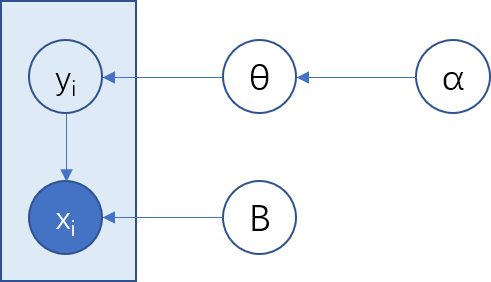
\includegraphics{./figure/bayesian.png}
    \caption{EM+Bayesian概率图
    \label{fig:bay}}
\end{figure*}


\begin{algorithm}[htb]
\caption{EM+Bayesian}
\label{alg:EM+B}
\begin{algorithmic}[1]
\REQUIRE
X; \\
\ENSURE 
$\alpha$,B; \\
\REPEAT 
\STATE E-step: $\gamma_{ik}=P(y_i,\theta|x_i;\alpha,B)$
\STATE M-step: $\sum_{i=1}^N\int_{\theta} P(y_i,\theta) \log P(x_i,y_i,\theta|\alpha,B)d{\theta}$
\UNTIL 
\RETURN $\alpha$,B;
\end{algorithmic}
\end{algorithm}


\subsection{SeqModel+HMM}
隐马尔可夫模型:隐藏的马尔可夫链随机生成的状态的序列,称为\textbf{状态序列};
每个状态生成一个观测,而由此产生的观测的随机序列,称为\textbf{观测序列}。
序列的每一个位置又可以看作是一个时刻。

例如, $\mathrm{N}$ 个袋子,每个袋子中有 $\mathrm{M}$ 种不同颜色的球。选择一个袋子,取出一个球,得到球的颜色。
\begin{enumerate}
    \item 状态数为 $N$ (袋子的数量)
    \item 每个状态可能的符号数 $\mathrm{M}$ (不同颜色球的数目)
    \item 状态转移概率矩阵 $\mathrm{A}=a_{i j}$ (从一只袋子(状态 Si) 转向另一只袋子(状态 $\mathrm{Sj}$ ) 取球的概率)
    \item 从状态 $\mathrm{Sj}$ 观察到某一特定符号 $\mathrm{vk}$ 的概率分布矩阵为: $B=b_{j}(k)$ (从第 $\mathrm{j}$ 个袋子中取出第 $\mathrm{k}$ 种颜色的球的概率)
    \item 初始状态的概率分布为: $\pi=\pi_{i}$
\end{enumerate}

一般将一个隐马尔可夫模型记为: $\lambda=[\pi, A, B]$
需要确定以下三方面内容(三要素):
\begin{enumerate}
    \item 初始状态概率 $\pi$ : 模型在初始时刻各状态出现的概率,通常记为 $\pi=\left(\pi_{1}, \pi_{2}, \ldots, \pi_{N}\right), \pi_{i}$ 表示模型的初始状态为 $S_{i}$ 的概率.
    \item 状态转移概率 $\mathrm{A}$ : 模型在各个状态间转换的概率,通常记为矩阵 $\mathrm{A}\left[a_{i j}\right]$ ,其中 $a_{i j}$ 表示在任意时 刻 $\mathrm{t}$ ,若状态为 $\mathrm{Si}$ ,则在下一时刻状态为 $\mathrm{Sj}$ 的概率.
    \item 输出观测概率 B: 模型根据当前状态获得各个观测值的概率通常记为矩阵 $B=\left[\left(b_{i j}\right)\right]$ 。其中, $b_{i j}$ 表示在任意时刻 $\mathrm{t}$ ,若状态为 $S_{i}$ ,则观测值 $O_{j}$ 被获取的概率.
\end{enumerate}

相对于马尔可夫模型,隐马尔可夫只是多了一个各状态的观测概率
给定隐马尔可夫模型 $\lambda=[A, B, \pi] $,它按如下过程产生观测序列 $\{X 1, X 2,\ldots, X n\}$ :
\begin{enumerate}
    \item 设置 $t=1$ ,并根据初始状态概率 $\pi$ 选择初始状态 $Y_{1}$ ;
    \item 根据状态值和输出观测概率 B 选择观测变量取值 $X_{t}$;
    \item 根据状态值和状态转移矩阵 $\mathrm{A}$ 转移模型状态,即确定 $Y_{t+1}$ ;
\end{enumerate}

\subsubsection{概率计算问题}
给定模型$\lambda=[\pi, A, B]$和观测序列$O=(o_1,\ldots,o_T)$,计算在模型$\lambda$
下观测序列$O$出现的概率$P(O|\lambda)$

\textbf{1. 直接计算法}:
对所有可能的状态序列$I$求和
$$
\begin{aligned}
    P(O|\lambda)
    &=\sum_I P(O|I,\lambda)P(I|\lambda)\\
    &=\sum \pi_i a_{i_1 i_2}\ldots a_{i_{T-1}i_T} \quad b_{i_1}(O_1)\ldots  b_{i_T}(O_T)
\end{aligned}
$$

\section{Lecture 12}
Outline
\begin{itemize}
    \item Undirected Graphical Model
    \item Revisit: $\lambda$
    \item $\lambda ++$: Reinforcement Learning: An Introduction
\end{itemize}

\subsection{作业}
分别用MLE和EM算法求解含有隐变量$h$的无向图模型。


\subsubsection*{MLE}
首先,
\begin{equation}
    \nabla_\theta \sum_{i=1}^n\ln P(v_i; \theta) = \sum_{i=1}^n  \nabla_\theta \ln \sum_{h_i} P(v_i, h_i; \theta) \label{start_eq}
\end{equation}

对于 $\nabla_\theta \ln \sum_{h_i} P(v_i, h_i; \theta)$ 进行计算,有
\begin{equation}
    \frac{1}{\sum_{h_i} P(v_i, h_i; \theta)} \sum_{h_i} \nabla_\theta P(v_i, h_i; \theta) \label{mid_eq}
\end{equation}
我们可以先看$\ln P(v,h; \theta)$, 有
\begin{equation*}
    \ln P(v,h; \theta) = -E(v,h;\theta) - \ln Z(\theta)
\end{equation*}
关于$\theta$求导,有
\begin{equation*}
    \frac{1}{P(v, h; \theta)}  \nabla_\theta P(v, h; \theta) = -\nabla_{\theta} E(v,h;\theta) - \frac{1}{Z(\theta)}\nabla_\theta Z(\theta)
\end{equation*}
从而得到
\begin{equation*}
    \nabla_\theta P(v, h; \theta) = P(v, h; \theta) * (-\nabla_{\theta} E(v,h;\theta) - \frac{1}{Z(\theta)}\nabla_\theta Z(\theta))
\end{equation*}
可以将其代入 公式 \ref{mid_eq}, 从而有
\begin{equation}
    \begin{aligned}
        \frac{1}{\sum_{h_i} P(v_i, h_i; \theta)} \sum_{h_i} \nabla_\theta P(v_i, h_i; \theta)
        &= \frac{1}{\sum_{h_i} P(v_i, h_i; \theta)} \sum_{h_i} P(v_i, h_i; \theta)(-\nabla_{\theta} E(v_i,h_i;\theta) - \frac{1}{Z(\theta)}\nabla_\theta Z(\theta))
    \end{aligned}
    \label{third_eq}
\end{equation}
其中$\frac{1}{Z(\theta)}\nabla_\theta Z(\theta)$ 在第一个无向图模型问题中求过,如下
\begin{equation*}
    \begin{aligned}
        \frac{\nabla_\theta Z(\theta)}{Z(\theta)} 
        &= \iint \frac{exp\{-E(v,h;\theta)\}}{Z(\theta)}(-\nabla_\theta E(v,h;\theta)) dv dh   \\
        &= -\mathbb{E}_{(v,h)\sim P(v,h;\theta)}[\nabla_\theta E(v,h;\theta)]
    \end{aligned}
\end{equation*}
且它与$\sum_{h_i}$无关,同时,$\sum_{h_i}P(v_i,h_i;\theta)$可视为一个值,公式\ref{third_eq}可写作
\begin{equation}
    \begin{aligned}
    &- \frac{1}{\sum_{h_i}P(v_i, h_i;\theta)}\mathbb{E}_{(v,h)\sim P(v,h;\theta)}[\nabla_\theta E(v,h;\theta)]-\sum_{h_i}\frac{P(v_i, h_i;\theta)}{P(v_i; \theta)}\nabla_{\theta} E(v_i,h_i;\theta) \\
    &= - \frac{1}{\sum_{h_i}P(v_i, h_i;\theta)}\mathbb{E}_{(v,h)\sim P(v,h;\theta)}[\nabla_\theta E(v,h;\theta)] - \mathbb{E}_{P(h_i|v_i)}[\nabla_{\theta} E(v_i,h_i;\theta)] \\
    \end{aligned}
\end{equation}
对于单个样本$v_i$,
\begin{gather*}
    \nabla_aE(v,h;\theta) = -v \\
    \nabla_bE(v,h;\theta) = -h \\
    \nabla_cE(v,h;\theta) = -v^Th \\
\end{gather*}
则,
\begin{gather*}
    \mathbb{E}[\nabla_aE(v,h;\theta)] = -E[V] \\
    \mathbb{E}[\nabla_bE(v,h;\theta)] = -E[H] \\
    \mathbb{E}[\nabla_cE(v,h;\theta)] = -E[V^TH]  \\
\end{gather*}
同样,
\begin{gather*}
    \mathbb{E}[\nabla_aE(v_i,h_i;\theta)] = -v_i \\
    \mathbb{E}[\nabla_bE(v_i,h_i;\theta)] = -h_i \\
    \mathbb{E}[\nabla_cE(v_i,h_i;\theta)] = -v_i^T h_i \\
\end{gather*}
$\theta=(a,b,)$的更新公式为:

\begin{equation}
    \begin{gathered}
        a^{t+1} \leftarrow a^t - \alpha(E[V]-v_i) \\
        b^{t+1} \leftarrow b^t - \alpha(E[H]-h_i) \\
        c^{t+1} \leftarrow c^t - \alpha(E[V^T H] - v_i^Th_i) \\
    \end{gathered}
\end{equation}


\begin{algorithm}[htb]
    \caption{MLE: SGD for Undirected Graphical Model}
    \label{alg:A10_1}
    \begin{algorithmic}[1]
    \REQUIRE
    $D=\{v_i\}_{i=1}^n$;\\
    \ENSURE 
    $\Theta=(a,b,C)$; \\
    \STATE init: $a,b,C$
    \REPEAT 
    \STATE $a^{t+1} \leftarrow a^t - \alpha(E[V]-v_i)$
    \STATE $b^{t+1} \leftarrow b^t - \alpha(E[H]-h_i)$
    \STATE $c^{t+1} \leftarrow c^t - \alpha(E[V^T H] - v_i^Th_i)$
    \UNTIL 
    \RETURN $\Theta$;
    \end{algorithmic}
\end{algorithm}

\subsubsection*{EM算法}
根据 公式\ref{start_eq} , 有
\begin{equation*}
    \ln \sum_{h_i} P(v_i, h_i; \theta)
    = \ln \sum_{h_i} P(h_i | v_i; \theta) \frac{P(v_i, h_i; \theta)}{P(h_i | v_i; \theta)}
\end{equation*}
其中,
\begin{equation*}
    \sum_{h_i} P(h_i | v_i; \theta) \frac{P(v_i, h_i; \theta)}{P(h_i | v_i; \theta)} = \mathbb{E}_{h_i\sim P(h_i|v_i;\theta)}[P(v_i|h_i;\theta)]
\end{equation*}
根据Jensen不等式,有
\begin{equation}
    \begin{aligned}
        \ln \mathbb{E}_{h_i\sim P(h_i|v_i;\theta)}[P(v_i|h_i;\theta)] 
        &\leq \mathbb{E}_{h_i\sim P(h_i|v_i;\theta)}[\ln P(v_i|h_i;\theta)]  \\
        &= \sum_{h_i}  P(h_i | v_i; \theta) \ln \frac{P(v_i, h_i; \theta)}{P(h_i | v_i; \theta)} \\
        &= \sum_{h_i} P(h_i | v_i; \theta) (\ln P(v_i,h_i;\theta) - \ln P(h_i | v_i; \theta)) \\
        &= \sum_{h_i} P(h_i | v_i; \theta)(\ln \frac{1}{Z(\theta)} \exp \{-E(v_i,h_i;\theta)\}) - P(h_i | v_i; \theta)\ln P(h_i | v_i; \theta) \\
        &= \sum_{h_i} P(h_i | v_i; \theta)(-E(v_i,h_i;\theta) -\ln Z(\theta)) - P(h_i | v_i; \theta)\ln P(h_i | v_i; \theta) \\
    \end{aligned} 
    \label{jensen_eq}
\end{equation}

\textbf{E-step}

对$P(h_i | v_i; \theta)$ 求导,构造拉格朗日乘子,
\begin{equation*}
    \mathcal{L}(P(h_i | v_i; \theta), \lambda) = \sum_{h_i} P(h_i | v_i; \theta)(-E(v_i,h_i;\theta) -\ln Z(\theta)) - P(h_i | v_i; \theta)\ln P(h_i | v_i; \theta) - \lambda(\sum_{h_i} P(h_i | v_i; \theta)-1)
\end{equation*}
对$P(h_i | v_i; \theta)$ 求导,有
\begin{equation*}
    \nabla_{P(h_i | v_i; \theta)} \mathcal{L}(P(h_i | v_i; \theta), \lambda)  = -E(v_i,h_i;\theta) -\ln Z(\theta)-\ln P(h_i | v_i; \theta)-1 -\lambda = 0
\end{equation*}
则, 
\begin{equation*}
    P(h_i | v_i; \theta)*\exp\{1+\lambda\} = \exp\{-E(v_i,h_i;\theta) -\ln Z(\theta) \}
\end{equation*}
因为$\sum_{h_i} P(h_i | v_i; \theta) = 1$, 因此
\begin{equation*}
    \sum_{h_i} P(h_i | v_i; \theta)* \exp\{1+\lambda\} = \sum_{h_i}\exp\{-E(v_i,h_i;\theta) -\ln Z(\theta) \}
\end{equation*}
从而,
\begin{equation*}
    \exp\{1+\lambda\} = \sum_{h_i}\exp\{-E(v_i,h_i;\theta) -\ln Z(\theta) \}
\end{equation*}
所以,
\begin{equation*}
    P(h_i | v_i; \theta) = \frac{exp\{-E(v_i,h_i;\theta) -\ln Z(\theta) \}}{\sum_{h_i}\exp\{-E(v_i,h_i;\theta) -\ln Z(\theta) \}}
\end{equation*}



\textbf{M-step}

根据 公式\ref{jensen_eq},对$\theta$求导,先分别求各项对$\theta$的求导结果
\begin{gather*}
    \nabla_aE(v_i,h_i;\theta) = -v_i \\
    \nabla_bE(v_i,h_i;\theta) = -h_i \\
    \nabla_cE(v_i,h_i;\theta) = -v_i^Th_i \\
    \\
    \begin{aligned}
        \frac{\nabla_\theta Z(\theta)}{Z(\theta)} 
        &= \iint \frac{exp\{-E(v,h;\theta)\}}{Z(\theta)}(-\nabla_\theta E(v,h;\theta)) dv dh   \\
        &= -\mathbb{E}_{(v,h)\sim P(v,h;\theta)}[\nabla_\theta E(v,h;\theta)]
    \end{aligned}
\end{gather*}
则求导结果为
\begin{gather*}
    \nabla_a(\cdot) = \sum_{h_i} P(h_i | v_i; \theta) v_i - E[V] = v_i - E[V] \\
    \nabla_b(\cdot) = \sum_{h_i} P(h_i | v_i; \theta) h_i - E[H] = \mathbb{E}_{h_i\sim P(h_i|v_i;\theta)}[h_i] - E[H] \\
    \nabla_c(\cdot) = \sum_{h_i} P(h_i | v_i; \theta) v_i^Th_i - E[V^TH] = \mathbb{E}_{h_i\sim P(h_i|v_i;\theta)}[v_i^Th_i] - E[V^TH] \\
\end{gather*}

\begin{algorithm}[htb]
    \caption{EM: SGD for Undirected Graphical Model}
    \label{alg:A10_2}
    \begin{algorithmic}[1]
    \REQUIRE
    $D=\{v_i\}_{i=1}^n$;\\
    \ENSURE 
    $\Theta=(a,b,C)$; \\
    \STATE init: $a,b,C$
    \REPEAT 
    \STATE \textbf{E-step}
    \STATE \quad \quad $P(h_i | v_i; \theta) = \frac{exp\{-E(v_i,h_i;\theta) -\ln Z(\theta) \}}{\sum_{h_i}\exp\{-E(v_i,h_i;\theta) -\ln Z(\theta) \}}$
    \STATE \textbf{M-step}
    \STATE \quad \quad $a^{t+1} \leftarrow a^t - \alpha(E[V]-v_i)$
    \STATE \quad \quad $b^{t+1} \leftarrow b^t - \alpha(E[H]-\mathbb{E}_{h_i\sim P(h_i|v_i;\theta)}[h_i])$
    \STATE \quad \quad $c^{t+1} \leftarrow c^t - \alpha(E[V^T H] - \mathbb{E}_{h_i\sim P(h_i|v_i;\theta)}[v_i^Th_i])$
    \UNTIL 
    \RETURN $\Theta$;
    \end{algorithmic}
\end{algorithm}


\end{document}



